\documentclass[12pt,a4paper]{article}

% ─── Packages ───────────────────────────────────────────────────────────────
\usepackage[margin=1in]{geometry}
\usepackage{amsmath,amssymb,amsthm}
\usepackage{physics}
\usepackage{braket}
\usepackage{graphicx}
\usepackage{hyperref}
\usepackage{cleveref}
\usepackage{enumitem}
\usepackage{booktabs}
\usepackage{xcolor}
\usepackage{tcolorbox}
\usepackage{fancyhdr}
\usepackage{titlesec}
\usepackage{setspace}
\usepackage{microtype}
\usepackage{titlesec}
\usepackage{float}
\usepackage{caption}
\usepackage{subcaption}
\usepackage{listings}
\usepackage[backend=biber,style=numeric,sorting=none]{biblatex}
\addbibresource{ref.bib}

% ─── Colors ─────────────────────────────────────────────────────────────────
\definecolor{mitred}{RGB}{163,31,52}
\definecolor{deepblue}{RGB}{0,33,99}
\definecolor{lightgray}{RGB}{240,240,240}
\definecolor{codegreen}{rgb}{0,0.6,0}
\definecolor{codegray}{rgb}{0.5,0.5,0.5}
\definecolor{codepurple}{rgb}{0.58,0,0.82}
 

% ─── Theorem Environments ────────────────────────────────────────────────────
\newtheorem{theorem}{Theorem}[section]
\newtheorem{corollary}[theorem]{Corollary}
\newtheorem{lemma}[theorem]{Lemma}
\newtheorem{definition}{Definition}[section]
\newtheorem{remark}{Remark}[section]

% ─── Custom Environments ────────────────────────────────────────────────────
\newenvironment{acknowledgements}{
    \begin{center}
        \textbf{Acknowledgements}
    \end{center}
    \small
}{}


% ─── Custom tcolorbox styles ─────────────────────────────────────────────────
\tcbuselibrary{skins,breakable}

\newtcolorbox{notebox}[1][]{
  enhanced, breakable,
  colback=blue!5!white, colframe=deepblue,
  title={\textbf{Background Note}},
  fonttitle=\small\bfseries,
  #1
}

\newtcolorbox{keyresult}[1][]{
  enhanced,
  colback=mitred!5!white, colframe=mitred,
  title={\textbf{Key Result}},
  fonttitle=\small\bfseries,
  #1
}

% ─── Code listing style ──────────────────────────────────────────────────────
\lstdefinestyle{pythonstyle}{
  backgroundcolor=\color{lightgray},
  commentstyle=\color{codegreen},
  keywordstyle=\color{deepblue}\bfseries,
  numberstyle=\tiny\color{codegray},
  stringstyle=\color{codepurple},
  basicstyle=\ttfamily\footnotesize,
  breakatwhitespace=false,
  breaklines=true,
  captionpos=b,
  keepspaces=true,
  numbers=left,
  numbersep=5pt,
  showspaces=false,
  showstringspaces=false,
  showtabs=false,
  tabsize=2,
  language=Python
}

% ─── Header/Footer ───────────────────────────────────────────────────────────
\pagestyle{fancy}
\fancyhf{}
\fancyhead[L]{\small\textcolor{deepblue}{Quantum State Discrimination}}
\fancyhead[R]{\small\textcolor{deepblue}{Term Paper}}
\fancyfoot[C]{\thepage}
\renewcommand{\headrulewidth}{0.4pt}

% ─── Section formatting ──────────────────────────────────────────────────────
\titleformat{\section}{\large\bfseries\color{deepblue}}{\thesection}{1em}{}[\titlerule]
\titleformat{\subsection}{\normalsize\bfseries\color{mitred}}{\thesubsection}{1em}{}

% ─── Spacing ─────────────────────────────────────────────────────────────────
\onehalfspacing

% ═══════════════════════════════════════════════════════════════════════════
\begin{document}

% ─── Title Page ──────────────────────────────────────────────────────────────
\begin{titlepage}
    \centering
    \vspace*{1.5cm}
    {\Huge\bfseries\color{deepblue}
        Quantum State Discrimination\\[0.2em]
        with Bosonic Channels\\[0.2em]
        and Gaussian States\\[1em]}
    {\large \textbf{Course}: PH3203 Advanced Quantum Mechanics\\}
    {\large \textbf{Instructor}: Professor Sourin Das\\}

    {\large\color{mitred}\rule{0.5\linewidth}{2pt}\\[1em]}
    {\large A Term Paper Review of Chapters 1--3\cite{mainref}\\[0.3em]
    \textit{Based on the MIT Doctoral Thesis by Si Hui Tan (2010)}\\[2em]}
    \begin{table}[H]
        \centering
        \caption*{\textbf{Authors}}
        \begin{tabular}{cc}
            Sapnodip Pramanik & Bikash Jyoti Saharia\\
            23MS145 & 23MS133 \\
            & \\
            Bhargab Neog & Shounak Goswami\\
            23MS177 & 23MS158
        \end{tabular}
    \end{table}
    \begin{figure}[H]
        \centering
        
\includegraphics[width=0.15\linewidth]{figures/logo.png}
    \end{figure}


    \vfill
    {\large\today \\}
    \vspace{0.5cm}
	{\large \textsc{INDIAN INSTITUTE OF SCIENCE EDUCATION AND RESEARCH, KOLKATA}\par}
    \newpage
    \begin{acknowledgements}
        [ACKNOWLEDGEMENT]
    \end{acknowledgements}
    \newpage
    \begin{abstract}
        \centering
        \noindent
            [ABSTRACT]
    \end{abstract}
\end{titlepage}



\tableofcontents
\newpage

\section{Introduction}
	\subsection{The notion of a quantum state}

A quantum state represented by a positive Hermitian operator $\hat{\rho}$ with unit trace, contains all physically relevant information about a quantum system. If two quantum systems are prepared in identical states, any measurement performed on them will yield identical outcome probabilities, making the different preparation methods observationally equivalent. Conversely, if the systems are in different quantum states, there necessarily exists at least one measurement that produces different probability distributions, allowing their preparations to be distinguished. The systematic process of designing and performing measurements to identify which of several possible states (and thus which preparation) a given system is in is called quantum state discrimination. 

\subsection{Measuring a quantum state}

While the quantum state itself is an abstract mathematical object, measurements provide it with concrete operational meaning. The outcomes of quantum measurements are always classical, such as a photodetector click count or an ion’s position in a trap, and these outcomes behave as random variables. By performing the same measurement many times on identically prepared quantum systems, one can reconstruct the statistical distribution of outcomes. If this process is repeated for every possible measurement, the complete set of outcome probability distributions fully characterizes the quantum state. Thus, the state is not directly observable, but its empirical reality is revealed through the statistics of measurement outcomes, bridging the gap between abstract formalism and experimental practice. The formal relationship between quantum states and measurements is captured by the postulates of standard quantum measurement theory. These postulates can be summarized as follows:

\begin{enumerate}
    \item Every physical observable corresponds to a Hermitian operator $\hat{X}$ with a spectral decomposition
    \begin{equation}
        \hat{X} = \sum_j \lambda_j |j\rangle\langle j|
    \end{equation}
    where $\lambda_j$ are the possible measurement outcomes.

    \item The projectors 
    \begin{equation}
        P_j = |j\rangle\langle j|
    \end{equation}
     associated with the eigenstates form a complete set, satisfying 
     \begin{equation}
         \sum_j P_j = \mathbb{I}
     \end{equation} and are orthogonal such that 
     \begin{equation}
         P_i P_j = \delta_{ij} P_i
     \end{equation}
     
    \item A measurement of $\hat{X}$ yields one of its eigenvalues $\lambda_j$ as the result.

    \item If the outcome $\lambda_j$ is obtained, the system collapses to the post-measurement state 
    \begin{equation}
        \hat{\rho}_j = \frac{P_j \hat{\rho} P_j}{\operatorname{tr}(P_j \hat{\rho} P_j)}
    \end{equation}

    \item The probability of obtaining the outcome $\lambda_j$ is given by 
    \begin{equation}
    p_j = \operatorname{tr}(\hat{\rho} P_j)    
    \end{equation}
    
    \item When the measurement is performed but the outcome is not recorded, the post-measurement state is described by the density operator 
    \begin{equation}
        \hat{\rho}' = \sum_j P_j \hat{\rho} P_j
    \end{equation}
     representing an average over all possible outcomes.
\end{enumerate}

It is important to note that in stating the postulates, the Hilbert space has been assumed to be finite and discrete solely for the sake of notational simplicity. In principle, these postulates apply equally to states with infinite-dimensional Hilbert spaces, which is precisely the case for continuous variable systems. The postulates make it clear that the measurement process is fundamentally random, with the outcome able to take a range of values. The number of possible measurement outcomes is equal to the dimension of the Hilbert space of the state. The projection operators $P_j$ used in this formulation are referred to as projective measurements or von Neumann measurements. However, it turns out that the requirement that measurement operators be strictly projective can be relaxed while still maintaining a meaningful statistical distribution for the outcomes. In particular, Postulate 3 provides an algorithm for generating outcome probabilities. \\

If we replace the projective measurement operator $P_j$ with a positive operator $\Pi_j$ that may not necessarily be a projection, the probability of obtaining outcome $j$ is given by 
\begin{equation}
    p_j = \operatorname{tr}(\hat{\rho} \Pi_j)
\end{equation}
 Since $\Pi_j$ is a positive operator, $p_j \geq 0$, and if we further require that the set of such operators for a finite set of outcomes is complete, meaning $\sum_j \Pi_j = \mathbb{I}$, then the quantities $p_j$ can be interpreted as probabilities for the outcomes of the measurement described by the operator set $\{\Pi_j\}$. Such a set of measurement operators is called a positive operator valued measure, or POVM. A key feature of POVMs is that their elements do not need to be orthogonal. Consequently, the number of possible outcomes can be larger than the dimension of the Hilbert space of the state being measured, offering greater flexibility in measurement design.\\

 Using POVMs, we can replace the postulates of the quantum theory of standard measurements with the following more flexible ones:

\begin{enumerate}
    \item Measurement operators are positive operators $\Pi_j \geq 0$ where the set of all such operators is complete: $\sum_j \Pi_j = \mathbb{I}$. The set of such operators is called a POVM. The elements of the POVM can be written in terms of generalized measurement operators $A_j$, where 
    \begin{equation}
        \Pi_j = A_j^\dagger A_j
    \end{equation}
     The generalized measurement operators can be non-Hermitian, though the elements of the POVM must be Hermitian by construction.
    
    \item Each element of the POVM set represents a possible outcome of the measurement.
    
    \item The state of the system after the measurement is
    \begin{equation}
    \hat{\rho}_j = \frac{A_j \hat{\rho} A_j^\dagger}{\operatorname{tr}(A_j \hat{\rho} A_j^\dagger)}    
    \end{equation}

    
    \item The probability that the outcome $j$ (indexing the measurement operator $\Pi_j$) is found is 
    \begin{equation}
    p_j = \operatorname{tr}(\Pi_j \hat{\rho})    
    \end{equation}
    
    
    \item If we perform the measurement but do not record the results, the post-measurement state is described by the density operator 
    \begin{equation}
    \hat{\rho}' = \sum_j A_j \hat{\rho} A_j^\dagger    
    \end{equation}
    
\end{enumerate}

The POVM formalism described above provides a way to describe classical information obtained from a quantum state by way of a measurement. State discrimination is the process of processing this information to determine, to the best of our knowledge, which quantum state we possess. The fundamental question of how well we can discriminate between quantum states lies at the heart of quantum mechanics. When the set of possible states are orthogonal to one another, perfect discrimination is always possible. This can be achieved by choosing a set of projection operators that correspond exactly to the set of possible states. However, when the possible states are non-orthogonal, perfect discrimination is impossible. In such cases, we must define optimal discrimination with respect to some figure of merit, though finding this optimal discrimination is often non-trivial. The chapter will next set up the problem of state discrimination and describe two commonly used strategies: minimum-error discrimination and unambiguous discrimination. Following that, some interesting well-known measurements that do not fall into these two categories, such as the pretty-good measurement and the no-measurement strategy, will be discussed.

\subsection{State Discrimination}
Consider an ensemble of quantum systems such that each system is prepared in one of $N$ possible states, say $\hat{\rho}_1, \ldots, \hat{\rho}_N$, with a priori probabilities $p_1, \ldots, p_N$ respectively, where $\sum_{j=1}^N p_j = 1$. In general, the states can be pure or mixed, and they can be either discrete variable states or continuous variable states. The observer performing state discrimination has full knowledge of the ensemble being prepared, meaning he knows the possible states and their prior probabilities. However, he does not know which one of the $N$ states he possesses, and he must make a measurement to determine this. State discrimination describes how he should design and perform these measurements to optimally identify the unknown state.\\

There are two commonly used strategies for state discrimination. The first is discrimination with minimum error, attributed to Helstrom, who studied distinguishing between two given quantum states. Helstrom found an optimum measurement strategy for both mixed and pure states that minimizes the probability of error. This optimum measurement strategy is known as the Helstrom measurement, and the resulting minimum error is called the Helstrom bound. The general problem of discriminating between $N>2$ states with minimum error is considerably more difficult. Although the necessary and sufficient conditions for an optimal measurement have been found, how to implement such an optimal measurement remains an open problem, except for a few special cases.\\

The second strategy is unambiguous discrimination, first proposed by Ivanovic. This strategy allows perfect discrimination between two non-orthogonal states, but with the caveat that a non-conclusive (inconclusive) answer is permitted. The specific case of discriminating between two pure non-orthogonal states was solved by Dieks and Peres. However, the general case of unambiguously discriminating between $N$ pure states remains an open problem. It has been shown by Chefles that unambiguous discrimination is only possible if the states to be distinguished are linearly independent. Additionally, there are active research areas focused on extending unambiguous discrimination strategies to mixed states.\\

Having described the two strategies briefly, let us now discuss each of them in more detail.

\subsubsection{State Discrimination with Minimum Error}
In the minimum error discrimination strategy, we always reach a conclusion about which state was prepared, though errors in this conclusion are inevitable. The goal of the optimal strategy is to minimize the detection error. To formulate this as a definite optimization problem, we must define what constitutes a detection error. \\

Let $\Pi_j$ be the POVM element corresponding to the state $\hat{\rho}_j$ being prepared. According to the postulates of quantum measurement theory, if the actual prepared state is $\hat{\rho}$, the probability of guessing that the state is $\hat{\rho}_j$ is $\operatorname{tr}(\hat{\rho} \Pi_j)$. Since the state $\hat{\rho}_j$ occurs with a priori probability $p_j$, the overall probability of a correct guess is given by 
\begin{equation}
    P_{\text{corr}} = \sum_{j=1}^N p_j \operatorname{tr}(\hat{\rho}_j \Pi_j)
\end{equation}
The detection error is then defined as 
\begin{equation}
    P_{\text{err}} = 1 - P_{\text{corr}}
\end{equation}
To minimize the error, we must minimize $P_{\text{err}}$ over all possible sets of POVM elements $\{\Pi_j\}$ for $j = 1, \ldots, N$ subject to the constraints $\Pi_j \geq 0$ and $\sum_{j=1}^N \Pi_j = \mathbb{I}$. The POVM that achieves this minimization is called the optimal measurement, and the resulting error is the minimum error. The special case of distinguishing single copies of two mixed states will be derived later in Section 3.3.1.

\subsubsection{Unambiguous State Discrimination}
Unlike discrimination with minimum error, in unambiguous discrimination we are not permitted to make measurement errors. However, this strategy does not succeed 100\% of the time, and this trade-off is necessary to achieve error-free discrimination.\\

To illustrate how unambiguous state discrimination works, we consider a simple example involving two pure states $|\psi_0\rangle$ and $|\psi_1\rangle$ occurring with equal a priori probabilities, given by

\begin{equation}
    |\psi_0\rangle = \cos\theta |0\rangle + \sin\theta |1\rangle
\end{equation}
\begin{equation}
    |\psi_1\rangle = \cos\theta |0\rangle - \sin\theta |1\rangle
\end{equation}

These states are non-orthogonal with overlap $\langle\psi_0|\psi_1\rangle = \cos^2\theta - \sin^2\theta = \cos(2\theta)$.\\

A POVM for distinguishing between these states can be constructed with elements

\begin{equation}
    \Pi_0 = a_0(\sin\theta |0\rangle + \cos\theta |1\rangle)(\sin\theta |0\rangle + \cos\theta |1\rangle)
\end{equation}
\begin{equation}
    \Pi_1 = a_1(\sin\theta |0\rangle - \cos\theta |1\rangle)(\sin\theta |0\rangle - \cos\theta |1\rangle)
\end{equation}
\begin{equation}
    \Pi_2 = \mathbb{I} - \Pi_0 - \Pi_1
\end{equation}

where the coefficients are chosen such that

\begin{equation}
    \langle\psi_0|\Pi_1|\psi_0\rangle = \langle\psi_1|\Pi_0|\psi_1\rangle = 0
\end{equation}

and $0 \leq a_0, a_1 \leq 1$. When outcome 0 is obtained, we can confidently conclude the state is $|\psi_0\rangle$; when outcome 1 is obtained, we can confidently conclude the state is $|\psi_1\rangle$. However, if outcome 2 occurs, no definite conclusion can be made.\\

To evaluate how effective this unambiguous discrimination strategy is, we need to determine the probability that the measurement yields an inconclusive result. A lower probability of inconclusive outcomes indicates a better discrimination scheme. Therefore, we now derive this probability and then optimize it over the available parameters. We begin by computing the conclusive probabilities. we first compute the conclusive probabilities. The probability of obtaining outcome 0 when $|\psi_0\rangle$ is sent is

\begin{equation}
    \langle\psi_0|\Pi_0|\psi_0\rangle = a_0 |\langle\psi_0|(\sin\theta |0\rangle + \cos\theta |1\rangle)|^2
\end{equation}

The overlap is

\begin{equation}
    \langle\psi_0|(\sin\theta |0\rangle + \cos\theta |1\rangle) = \cos\theta\sin\theta + \sin\theta\cos\theta = \sin(2\theta)
\end{equation}

Thus,

\begin{equation}
    \langle\psi_0|\Pi_0|\psi_0\rangle = a_0 \sin^2(2\theta)
\end{equation}

Similarly, for $|\psi_1\rangle$,

\begin{equation}
    \langle\psi_1|\Pi_1|\psi_1\rangle = a_1 \sin^2(2\theta)
\end{equation}

Since the prior probabilities are equal ($p_0 = p_1 = 1/2$), the overall probability of a conclusive result is

\begin{equation}
    P_{\text{conc}} = \frac{1}{2} a_0 \sin^2(2\theta) + \frac{1}{2} a_1 \sin^2(2\theta)
\end{equation}

Completeness of the POVM and positivity of $\Pi_2$ imposes constraints on $a_0$ and $a_1$. The optimal choice that maximizes the conclusive probability (or equivalently minimizes the inconclusive probability) is found to be $a_0 = a_1 = 1/(1 + \cos(2\theta))$. Substituting this value, we obtain

\begin{equation}
    \langle\psi_0|\Pi_0|\psi_0\rangle = \frac{\sin^2(2\theta)}{1 + \cos(2\theta)} = \frac{1 - \cos^2(2\theta)}{1 + \cos(2\theta)} = 1 - \cos(2\theta)
\end{equation}

Thus, the probability of obtaining an inconclusive result when $|\psi_0\rangle$ is sent is $1 - (1 - \cos(2\theta)) = \cos(2\theta)$. The same holds for $|\psi_1\rangle$. Therefore, the overall probability of an inconclusive result is

\begin{equation}
    P(\text{inconclusive result}) = \cos(2\theta)
\end{equation}

This minimum value is known as the Ivanovic-Dieks-Peres (IDP) limit. Analytical solutions for the IDP limit are not known for the general case of $N > 2$ pure states, though the solution for three pure states has been derived. Various numerical techniques have also been developed to calculate the IDP limit in the general case.

\subsubsection{Pretty-Good Measurement}
More often than not, in minimum-error state discrimination, it is not possible to find the optimal measurement. In such cases, the pretty-good measurement (PGM), also known as the square-root measurement, is---as its name suggests---a good measurement strategy to pursue. For a given set of $N$ possible states, we can always construct the POVM elements of the PGM as 
\begin{equation}
    \hat{\Pi}_i = p_i \hat{\rho}^{-1/2} \hat{\rho}_i \hat{\rho}^{-1/2} \text{ for } i = 1, \ldots, N
\end{equation}
where 
\begin{equation}
    \hat{\rho} = \sum_i p_i \hat{\rho}_i
\end{equation}
and $p_i$ is the probability of the $i$th state $\hat{\rho}_i$ occurring. The POVM elements defined in this way satisfy both positivity and completeness. Although the PGM is not the optimal measurement in the general case, it turns out to be optimal for many of the cases in which the minimum-error measurement is known. These results have been summarized in the literature.

\subsubsection{Other Measurement Strategies}
An interesting state discrimination strategy is the no-measurement strategy. For some sets of states, the optimal measurement is to make no measurements at all and simply guess the state that is most likely. A practical example where the no-measurement strategy applies is distinguishing a state from random noise: if the signal-to-noise ratio is sufficiently low, one should always guess that the received state was random noise.\\

Additionally, there exist mixed strategies that allow inconclusive results while minimizing the probability of detection error, as considered by Chefles and Barnett. The suggested potential use of such mixed strategies is to provide added flexibility for an eavesdropper to "listen in" on a cryptographic protocol.\\

Having discussed some of the strategies for state discrimination, important questions still remain: How does state discrimination help our understanding of quantum mechanics, and how can it be used in quantum protocols? The next section will address these questions.

\subsection{The Role of State Discrimination in Quantum
Information Theory}

\begin{figure}[H]
    \centering
    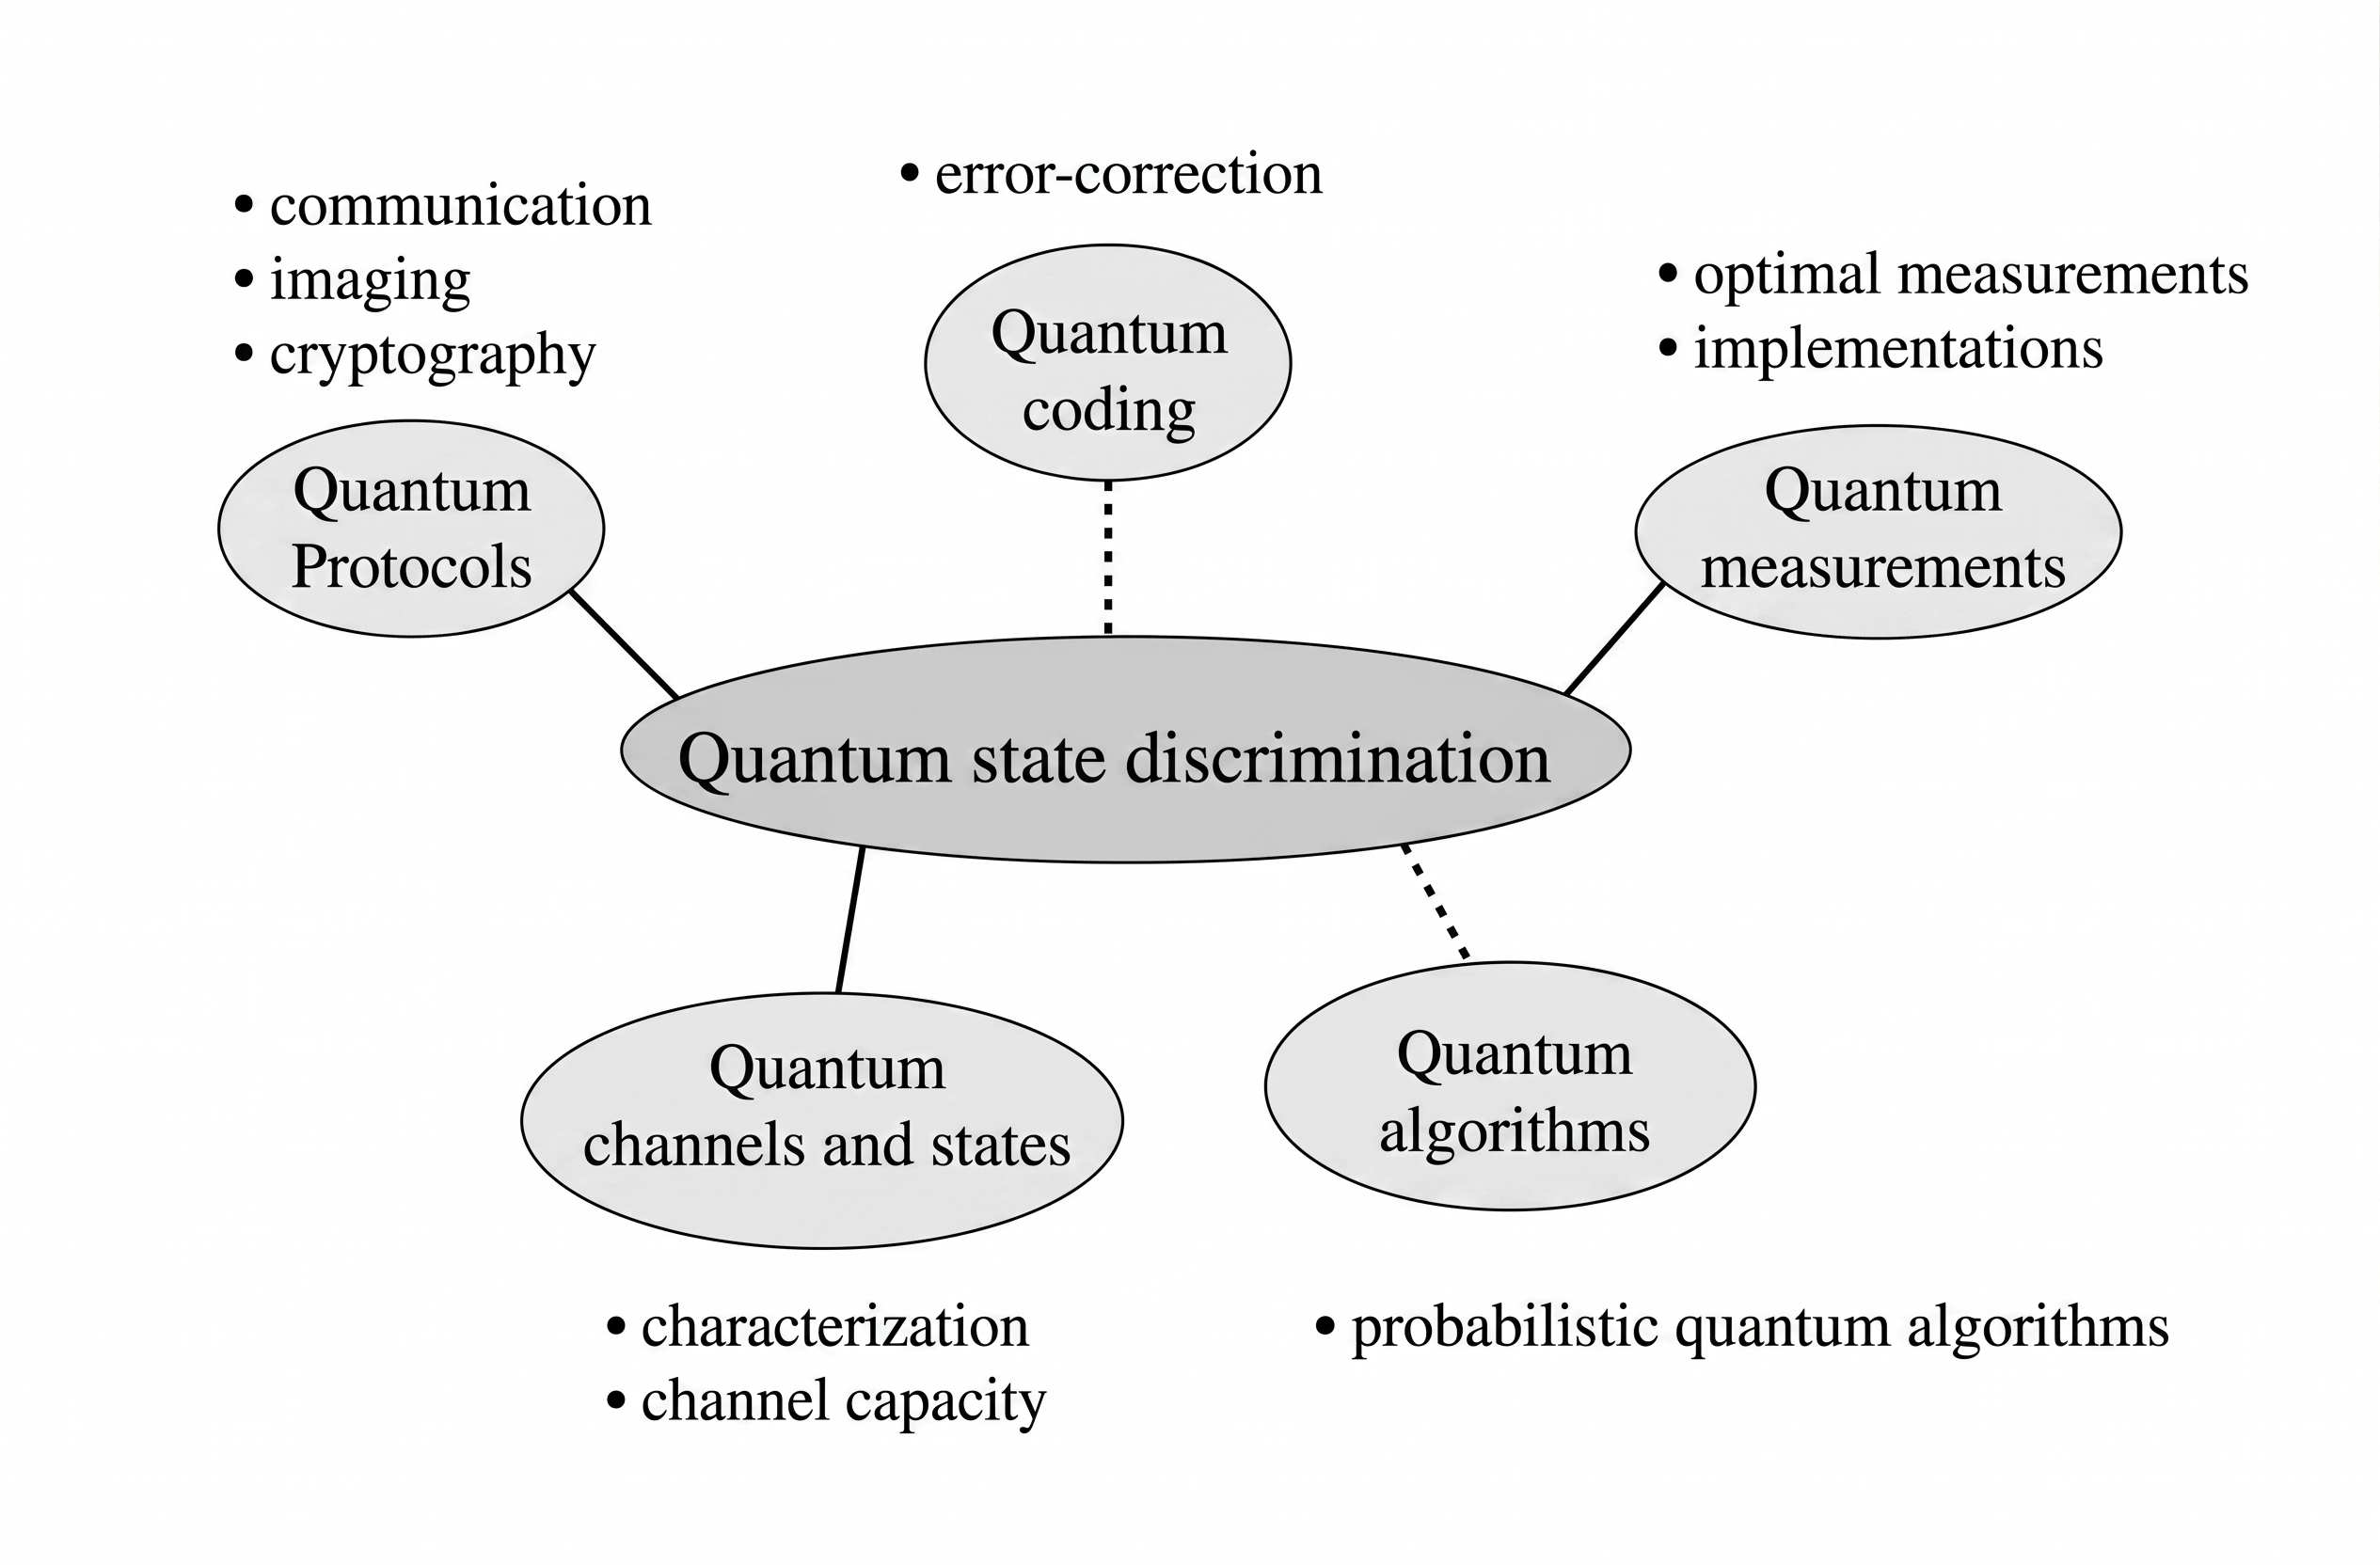
\includegraphics[width=1.0\textwidth]{figures/qsd.jpg}
    \caption{An overview of the central role of quantum state discrimination in quantum information theory.\cite{mainref}}
    \label{fig:qsd_overview}
\end{figure}

Quantum state discrimination lies at the heart of quantum computation and communication. The specific strategy of state discrimination applied depends on the task in quantum information theory to be solved. For example, using state discrimination techniques, we can show that quantum mechanics does not permit perfect discrimination between nonorthogonal states $|\psi_0\rangle$ and $|\psi_1\rangle$---a result that is also directly implied by the no-cloning theorem.\\

To demonstrate this, assume we have a POVM with two elements $\Pi_0$ and $\Pi_1$. For perfect discrimination, we require that

\begin{equation}
    \Pi_0 |\psi_1\rangle = 0
\end{equation}
\begin{equation}
\Pi_1 |\psi_0\rangle = 0
\end{equation}

This means that if outcome $0$ is obtained, we deduce the state was $|\psi_0\rangle$, and if outcome $1$ is obtained, we deduce the state was $|\psi_1\rangle$. The POVM operators must also satisfy the completeness relation

\begin{equation}
    \Pi_0 + \Pi_1 = \mathbb{I}
\end{equation}

To derive the necessary condition for perfect discrimination, we multiply the above equation on the left by $\langle\psi_0|$ and on the right by $|\psi_1\rangle$:

\begin{equation}
    \langle\psi_0| (\Pi_0 + \Pi_1) |\psi_1\rangle = \langle\psi_0| \mathbb{I} |\psi_1\rangle
\end{equation}

Distributing the left-hand side gives

\begin{equation}
    \langle\psi_0|\Pi_0|\psi_1\rangle + \langle\psi_0|\Pi_1|\psi_1\rangle = \langle\psi_0|\psi_1\rangle 
\end{equation}

Now, from the perfect discrimination conditions, we have $\Pi_0|\psi_1\rangle = 0$. Therefore, the first term $\langle\psi_0|\Pi_0|\psi_1\rangle = 0$. For the second term, note that $\Pi_1$ is a positive operator. If $\Pi_1|\psi_0\rangle = 0$, then taking the adjoint gives $\langle\psi_0|\Pi_1 = 0$. However, this does not directly imply $\langle\psi_0|\Pi_1|\psi_1\rangle = 0$. In standard unambiguous discrimination, the POVM elements are constructed such that $\Pi_1$ projects onto a subspace orthogonal to $|\psi_0\rangle$, which indeed forces $\langle\psi_0|\Pi_1|\psi_1\rangle = 0$. Under this construction, we have,

\begin{equation}
    0 + 0 = \langle\psi_0|\psi_1\rangle
\end{equation}

Thus,

\begin{equation}
    \langle\psi_0|\psi_1\rangle = 0 
\end{equation}

This condition can only be satisfied if the states $|\psi_0\rangle$ and $|\psi_1\rangle$ are orthogonal. Consequently, perfect discrimination is impossible for non-orthogonal states. Insights such as these are prevalent when applying state discrimination to problems in quantum information theory. The fact that we cannot perfectly distinguish between non-orthogonal states is what makes quantum key distribution possible.\\

Another important use of state discrimination is to characterize properties of quantum states, such as entanglement and separability. Much research has been devoted to this area. One of the main motivations behind such studies is to determine whether entangled states are useful for certain tasks, or whether entanglement is needed for a given task at all. Quantum metrology, quantum imaging, and the classical capacity of quantum channels are examples of such investigations.\\

State discrimination is also indispensable in quantum error correction. Error correction cannot be performed without syndrome measurement. A syndrome measurement determines whether a quantum state has been corrupted and, if so, which part of the state has been affected. The syndrome measurement is typically a multi-state measurement that does not disturb the encoded state but still provides information about the error. Such measurements lie at the heart of error correction.\\

Finally, state discrimination has found uses in quantum algorithms through a variant known as quantum state filtering. In quantum state filtering, the goal is to determine whether an unknown quantum state is a specific state $|\psi_k\rangle$ from a set of known states $\{|\psi_1\rangle, \ldots, |\psi_N\rangle\}$, or one of the others. Using optimal solutions in quantum state filtering, it is possible to implement an efficient probabilistic quantum algorithm that distinguishes between sets of Boolean functions, which generalizes the Deutsch-Jozsa algorithm. It has also been proposed that quantum decision problems can be characterized by state discrimination.\\

Having discussed the role of state discrimination in the major topics of quantum information theory, we now introduce the encoding of information onto continuous variable states.

\subsection{Continuous Variables in Quantum Mechanics}
While quantum information is primarily concerned with discrete quantum variables, such as qubits, continuous variable states have always played an important role in quantum mechanics. The position and momentum of the quantized harmonic oscillator are continuous variables. Because a mode of the electromagnetic field can be thought of as a harmonic oscillator, its quadrature amplitudes (the electric and magnetic fields) are continuous variables. Due to this connection to the quantized electromagnetic field, the development of the laser in the 1960s inspired considerable research into the properties of continuous quantum variables.\\

Continuous variables also play an important role in quantum information. The original EPR thought experiment was formulated in terms of the entangled momentum and position states of two particles. Furthermore, one of the first experimental demonstrations of quantum teleportation was performed using continuous variable states. Many aspects of discrete quantum information theory have continuous analogues, including quantum codes. It is even possible to formulate a theory of universal quantum computation over continuous variables by combining linear optical devices such as phase shifters and beamsplitters with nonlinear elements such as downconverters and parametric amplifiers.\\

The primary reason for developing a theory of quantum information over continuous variables is a practical one. Most communication channels involve the exchange of bosons (such as photons or phonons), which correspond to quantized harmonic oscillators. Accordingly, the theory of quantum information over continuous variables is essential for understanding the physical limits of communication. Moreover, many important sensing and measurement techniques, including microscopy and radar, rely on bosonic systems. Quantum information over continuous variables is the key to understanding the limits of sensing and measurement and for devising methods to attain those limits. With this motivation, this work explores the fundamental limits of quantum communication and sensing and introduces techniques to achieve them, beginning with a review of continuous variable quantum information theory in the following chapter.

\subsection{Scope of This Work}
This subsection lists the major research areas in continuous variable quantum computing and quantum information, and situate the contributions of this work within them.\\

Major areas of research include:

\begin{enumerate}
    \item \textbf{Channel Capacity of the Noisy, Lossy Bosonic Channel:} A fundamental question in quantum communication is: what is the maximum rate at which information can be sent down a bosonic channel in the presence of loss and noise? The capacity of a quantum channel $\mathcal{E}$ with inputs drawn from an ensemble of states $\hat{\rho}_k$ with probabilities $p_k$ is given by its Holevo quantity,

\begin{equation}
    \chi(\{p_k, \hat{\rho}_k\}) = S\left(\sum_k p_k \mathcal{E}(\hat{\rho}_k)\right) - \sum_k p_k S\left(\mathcal{E}(\hat{\rho}_k)\right),
\end{equation}

where $S(\hat{\rho})$ is the von Neumann entropy of the state $\hat{\rho}$. Maximizing this quantity over all possible ensembles, including entangled inputs across multiple uses of the channel, yields the channel capacity. This maximization is often difficult to perform. The capacity of the bosonic channel with linear loss is known and is attained by sending ensembles of coherent states down the channel. By contrast, the capacity of the bosonic channel with linear loss and thermal noise remains unknown, although it is conjectured to also be attained by sending ensembles of coherent states.

    \item \textbf{Minimum Output Entropy Conjecture:} The capacity of the bosonic channel with linear loss and thermal noise is indeed attained by coherent state inputs if the bosonic minimum output entropy conjecture holds. This conjecture states that a coherent-state input yields the output with the minimum von Neumann entropy for a bosonic channel with additive Gaussian noise. Proving or disproving the bosonic minimum output entropy conjecture is perhaps the most important open problem in continuous variable quantum information theory.

    \item \textbf{Optimal Measurements for Distinguishing Bosonic States:} Distinguishing quantum states is an important component of quantum information science. Key results, such as the no-cloning theorem, the quantum teleportation protocol, and more recently the Yuen no-go theorem, have their origins in problems of state discrimination. The Helstrom bound gives the minimum probability of error technique for discriminating between two quantum states. The quantum Chernoff bound is an upper bound to the Helstrom limit of multiple-copy binary state discrimination, which is asymptotically tight in the error exponent. While the measurement techniques for attaining the Helstrom bound are known in principle, devising experimentally practical measurement techniques for attaining the Helstrom bound is not known in general. Moreover, even when the channel capacity for a quantum channel is attained by product state (unentangled) inputs, the measurement required to attain the capacity is the entangling `pretty-good' measurement, which may be hard to perform in practice. For example, even though the channel capacity for the bosonic channel with linear loss is attained by coherent state inputs, practical decoding techniques that attain this bound are not currently known.

\end{enumerate}


\section{Continuous Variable Quantum Information Theory}
\subsection{Coherent States}

\subsubsection{Fock representation of the coherent state}


Assume that the annihilation operator $\hat{a}$ has a right eigenstate. Because $\hat{a}$ is not Hermitian, its eigenvalue will in general be some complex number $\alpha$, and we label the corresponding eigenstate $|\alpha\rangle$ by the same complex number $\alpha$. We may therefore write the equation
\begin{equation*} \hat{a}|\alpha\rangle=\alpha|\alpha\rangle. \end{equation*}

The conjugate state $\langle\alpha|$ is obviously a left eigenstate of the creation operator $\hat{a}^{\dagger}$, as can be seen by taking the Hermitian conjugate.
\begin{equation*} \langle\alpha|\hat{a}^{\dagger}=\alpha^{*}\langle\alpha|. \end{equation*}

The state $|\alpha\rangle$ will be called the coherent state. Our initial goal is to find an explicit representation for $|\alpha\rangle$ in the basis of Fock states $|n\rangle$ labelled by the occupation number $n$. Since the Fock states form a complete set, we may use them to represent $|\alpha\rangle$ in the form
\begin{equation*} |\alpha\rangle=\sum_{n=0}^{\infty}c_{n}|n\rangle, \end{equation*}
in which the $c_{n}$ are complex numbers to be determined. On substituting the expansion and using the "step down" equation, we obtain
\begin{equation*} \sum_{n=1}^{\infty}c_{n}\sqrt{n}|n-1\rangle=\alpha\sum_{n=0}^{\infty}c_{n}|n\rangle. \end{equation*}

As the $|n\rangle$ $(n=0,1,2,...)$ are a set of orthogonal state vectors, this equation is satisfied only if the coefficients of corresponding Fock state vectors on both sides are equal. We therefore have, on equating coefficients of $|n-1\rangle$,
\begin{equation*} c_{n}=\frac{\alpha}{\sqrt{n}}c_{n-1}. \end{equation*}

This is a recursion formula connecting $c_{n}$ and $c_{n-1}$ from which we obtain by repeated application
\begin{equation*} c_{n}=\frac{\alpha^{2}}{[n(n-1)]^{1/2}}c_{n-2}=...=\frac{\alpha^{n}}{\sqrt{n!}}c_{0}, \end{equation*}
so that
\begin{equation*} |\alpha\rangle=c_{0}\sum_{n=0}^{\infty}\frac{\alpha^{n}}{\sqrt{n!}}|n\rangle. \end{equation*}

$c_{0}$ can be determined from the requirement that the state $|\alpha\rangle$ be normalized to unity, which implies
\begin{align*}
\langle\alpha|\alpha\rangle &= 1=|c_{0}|^{2}\sum_{n=0}^{\infty}\sum_{m=0}^{\infty}\frac{\alpha^{*n}\alpha^{m}}{\sqrt{n!}\sqrt{m!}}\langle n|m\rangle \\
&= |c_{0}|^{2}\sum_{n=0}^{\infty}\frac{|\alpha|^{2n}}{n!} \\
&= |c_{0}|^{2}e^{|\alpha|^{2}},
\end{align*}
when we make use of the orthogonality of the Fock states. Hence
\begin{equation*} |c_{0}|=e^{-|\alpha|^{2}/2}, \end{equation*}
and, apart from a unimodular factor, we have
\begin{equation}
    |\alpha\rangle=e^{-|\alpha|^{2}/2}\sum_{n=0}^{\infty}\frac{\alpha^{n}}{\sqrt{n!}}|n\rangle, 
\end{equation}
and
\begin{equation*} \langle\alpha|=e^{-|\alpha|^{2}/2}\sum_{n=0}^{\infty}\frac{\alpha^{*n}}{\sqrt{n!}}\langle n|. \end{equation*}

It is interesting to note that for every complex number $\alpha$, other than zero, the coherent state $|\alpha\rangle$ has a non-zero projection on every Fock state $|n\rangle$. Thus
\begin{equation*} \langle n|\alpha\rangle=e^{-|\alpha|^{2}/2}\frac{\alpha^{n}}{\sqrt{n!}}. \end{equation*}

When $\alpha=0$, the coherent state $|\alpha\rangle$ becomes the vacuum state $|vac\rangle$, which may be regarded as either a coherent state or a Fock state. The squared modulus of the projection of $|\alpha\rangle$ onto $|n\rangle$ gives the probability $p(n)$ that $n$ excitations or photons will be found in the coherent state $|\alpha\rangle$. We therefore have
\begin{equation} p(n)=|\langle n|\alpha\rangle|^{2}=\frac{|\alpha|^{2n}}{n!}e^{-|\alpha|^{2}}, \end{equation}
which will be recognized as a Poisson distribution in $n$, with parameter $|\alpha|^{2}$. The mean number of photons present when the state is a coherent state $|\alpha\rangle$ is therefore given by(Poisson distbn - mean is the $\lambda$ of the distbn. - here  $|\alpha|^{2}$ ).
\begin{equation}
\sum_{n=0}^{\infty}np(n)=|\alpha|^{2}=\langle\alpha|\hat{a}^{\dagger}\hat{a}|\alpha\rangle 
\end{equation}
and this is large or small according as $\alpha$ is a large or small number.

{But, no matter how small $\alpha$ may be (with the exception of $\alpha=0$), there is some non-zero probability $p(n)$ that any number of photons $n$, however large, is present in the field. In a certain sense the photon number is as random as possible in a coherent state, subject to a certain mean number $|\alpha|^{2}$. It is a remarkable feature of the combination of Fock states that the state is unchanged when acted on by the annihilation operator $\hat{a}$. A possible connection between the coherent state of the quantum field and a classical field is suggested by the fact that it is possible to absorb photons from an electromagnetic field in a coherent state repeatedly, without changing the state in any way.}

{At first sight it might seem that, because the coherent state is not the eigenstate of any observable, it does not correspond to any readily measurable feature of the electromagnetic field. However, this is not so, because in practice most measurements of the field in the optical domain are based on the process of photoelectric detection. This includes instruments such as the photomultiplier, the photoconductor, the photographic plate and the eye. These instruments function by the absorption of photons, and it is therefore the absorption operator which is most closely associated with the measurement of the field. It is partly because the coherent states are eigenstates of the absorption operator, that these states prove to be particularly convenient for the description of many properties of the field encountered in photoelectric measurements.\cite[Chapter 11]{MandelWolf1995}

\subsubsection{The coherent state as a displaced vacuum state - the displacement operator}

By combining the expansion with the representation of the Fock state $|n\rangle = \frac{\hat{a}^{\dagger n}}{\sqrt{n!}}| vac\rangle$, we can write
\begin{align*}
|\alpha\rangle &= e^{-|\alpha|^{2}/2}\sum_{n=0}^{\infty}\frac{\alpha^{n}\hat{a}^{\dagger n}}{n!}|vac\rangle \\
&= e^{-|\alpha|^{2}/2}e^{\alpha\hat{a}^{\dagger}}|vac\rangle,
\end{align*}
which shows that the coherent state $|\alpha\rangle$ may also be regarded as a displaced vacuum state .

We can re-express this in a somewhat more symmetric form, by inserting the operator $e^{-\alpha^{*}\hat{a}}$ between $e^{\alpha\hat{a}^{\dagger}}$ and $|vac\rangle$. Thus

    


\begin{equation} |\alpha\rangle=e^{-|\alpha|^{2}/2}e^{\alpha\hat{a}^{\dagger}}e^{-\alpha^{*}\hat{a}}|vac\rangle. \end{equation}



The insertion of $e^{-\alpha^{*}\hat{a}}$ can be justified by expansion of the exponential operator, which leads to the result
\begin{align*}
e^{-\alpha^{*}\hat{a}}|vac\rangle &= \left[1-\alpha^{*}\hat{a}+\frac{(\alpha^{*}\hat{a})^{2}}{2!}-...\right]|vac\rangle \\
&= |vac\rangle.
\end{align*}

We now make use of the Campbell-Baker-Hausdorff operator identity for two operators $\hat{A}$, $\hat{B}$ provided that
\begin{equation*} \exp(\hat{A}+\hat{B})=\exp\hat{A}\exp\hat{B}\exp(-[\hat{A},\hat{B}]/2), \end{equation*}
\begin{equation*} [\hat{A},[\hat{A},\hat{B}]]=0=[\hat{B},[\hat{A},\hat{B}]]. \end{equation*}

The condition is obviously satisfied for any pair of operators $\hat{A}$, $\hat{B}$ whose commutator $[\hat{A}, \hat{B}]$ is a c-number. If we now put $\hat{A}=\alpha\hat{a}^{\dagger}$, $\hat{B}=-\alpha^{*}\hat{a}$ and make use of the commutation relation, we obtain $[\hat{A},\hat{B}]=|\alpha|^{2}$ and
\begin{equation*} e^{\alpha\hat{a}^{\dagger}-\alpha^{*}\hat{a}}=e^{\alpha\hat{a}^{\dagger}}e^{-\alpha^{*}\hat{a}}e^{-|\alpha|^{2}/2} \end{equation*}
which allows us to re-write the equation in the more compact form
\begin{equation} |\alpha\rangle=\hat{D}(\alpha)|0\rangle \label{eq:displacementoperator}, \end{equation}
where
\begin{equation*} \hat{D}(\alpha)\equiv e^{\alpha\hat{a}^{\dagger}-\alpha^{*}\hat{a}}. \end{equation*}

$\hat{D}(\alpha)$ is the displacement operator that creates the coherent state $|\alpha\rangle$ from the vacuum state $|0\rangle=|vac\rangle$. It is clear by inspection that $\hat{D}(\alpha)$ is a unitary operator such that
\begin{equation*} \hat{D}^{\dagger}(\alpha)\hat{D}(\alpha)=1=\hat{D}(\alpha)\hat{D}^{\dagger}(\alpha), \end{equation*}
and
\begin{equation*} \hat{D}^{\dagger}(\alpha)=\hat{D}(-\alpha). \end{equation*}


The displacement operator also has the following property:

{Unitary transformation of $\hat{a}$ or $\hat{a}^{\dagger}$ leads to the complex displacement $\alpha$ or $\alpha^{*}$, respectively. Thus
\begin{equation*} \hat{D}^{\dagger}(\alpha)\hat{a}\hat{D}(\alpha)=\hat{a}+\alpha \end{equation*}
and
\begin{equation*} \hat{D}^{\dagger}(\alpha)\hat{a}^{\dagger}\hat{D}(\alpha)=\hat{a}^{\dagger}+\alpha^{*}. \end{equation*} }

{These properties follow by applying the operator expansion theorem (the Hadamard lemma), which states that for any operators $\hat{A}$ and $\hat{B}$:}
\begin{equation*} e^{\hat{A}}\hat{B}e^{-\hat{A}} = \hat{B} + [\hat{A},\hat{B}] + \frac{1}{2!}[\hat{A},[\hat{A},\hat{B}]] + \dots \end{equation*}

{Letting the displacement operator be $\hat{D}(\alpha) = e^{\alpha\hat{a}^{\dagger}-\alpha^{*}\hat{a}}$, its adjoint is $\hat{D}^{\dagger}(\alpha) = e^{-\alpha\hat{a}^{\dagger}+\alpha^{*}\hat{a}}$. To map this to the theorem, we set $\hat{A} = -\alpha\hat{a}^{\dagger}+\alpha^{*}\hat{a}$. First, we evaluate the transformation of $\hat{B} = \hat{a}$. Using the fundamental commutation relations $[\hat{a},\hat{a}^{\dagger}]=1$ and $[\hat{a}^{\dagger},\hat{a}]=-1$, we compute the first-order commutator:}
\begin{align*}
[\hat{A},\hat{a}] &= [-\alpha\hat{a}^{\dagger}+\alpha^{*}\hat{a}, \hat{a}] \\
&= -\alpha[\hat{a}^{\dagger},\hat{a}] + \alpha^{*}[\hat{a},\hat{a}] \\
&= -\alpha(-1) + 0 \\
&= \alpha
\end{align*}

{Because $\alpha$ is a c-number (scalar), it commutes with all operators. Therefore, all higher-order nested commutators strictly vanish:}
\begin{equation*} [\hat{A},[\hat{A},\hat{a}]] = [\hat{A},\alpha] = 0 \end{equation*}

{Substituting these terms back into the expansion theorem, the infinite series truncates exactly after the second term:}
\begin{equation*} \hat{D}^{\dagger}(\alpha)\hat{a}\hat{D}(\alpha) = e^{-\alpha\hat{a}^{\dagger}+\alpha^{*}\hat{a}}\hat{a}e^{\alpha\hat{a}^{\dagger}-\alpha^{*}\hat{a}} = \hat{a} + \alpha \end{equation*}

We repeat the process for $\hat{B} = \hat{a}^{\dagger}$. The first-order commutator evaluates to:
\begin{align*}
[\hat{A},\hat{a}^{\dagger}] &= [-\alpha\hat{a}^{\dagger}+\alpha^{*}\hat{a}, \hat{a}^{\dagger}] \\
&= -\alpha[\hat{a}^{\dagger},\hat{a}^{\dagger}] + \alpha^{*}[\hat{a},\hat{a}^{\dagger}] \\
&= 0 + \alpha^{*}(1) \\
&= \alpha^{*}
\end{align*}

Once again, the resulting c-number $\alpha^{*}$ causes all higher-order nested commutators ($[\hat{A},\alpha^{*}]$) to vanish. The expansion truncates cleanly, yielding:
\begin{equation*} \hat{D}^{\dagger}(\alpha)\hat{a}^{\dagger}\hat{D}(\alpha) = e^{-\alpha\hat{a}^{\dagger}+\alpha^{*}\hat{a}}\hat{a}^{\dagger}e^{\alpha\hat{a}^{\dagger}-\alpha^{*}\hat{a}} = \hat{a}^{\dagger} + \alpha^{*} \end{equation*}
\cite[Chapter 11]{MandelWolf1995}

\subsection{Thermal States}

\subsubsection{The Density Matrix}
We begin with the fundamental postulate of statistical mechanics for a system in thermal equilibrium with a heat bath. The canonical ensemble defines the unnormalized density operator as $e^{-\beta\hat{H}}$, where $\beta = \frac{1}{k_B T}$ and $\hat{H}$ is the Hamiltonian. For a quantum harmonic oscillator, the Hamiltonian is $\hat{H} = \hbar\omega\left(\hat{a}^{\dagger}\hat{a} + \frac{1}{2}\right)$.

To find the normalized density operator $\hat{\rho}_{th}$, we divide by the partition function $Z$:
\begin{equation}
    \hat{\rho}_{th} = \frac{1}{Z} e^{-\beta\hbar\omega\left(\hat{a}^{\dagger}\hat{a} + 1/2\right)}
\end{equation}

We evaluate the partition function $Z$ by taking the trace over the Fock state basis $|n\rangle$:
\begin{align*}
    Z &= \text{Tr}\left(e^{-\beta\hat{H}}\right) \nonumber \\
      &= \sum_{n=0}^{\infty} \langle n| e^{-\beta\hbar\omega\left(\hat{a}^{\dagger}\hat{a} + 1/2\right)} |n\rangle \nonumber \\
      &= e^{-\frac{\beta\hbar\omega}{2}} \sum_{n=0}^{\infty} e^{-\beta\hbar\omega n}
\end{align*}

Because $e^{-\beta\hbar\omega} < 1$, we recognize this as a convergent geometric series $\sum_{n=0}^\infty x^n = \frac{1}{1-x}$. Evaluating the series yields:
\begin{equation*}
    Z = e^{-\frac{\beta\hbar\omega}{2}} \left( \frac{1}{1 - e^{-\beta\hbar\omega}} \right)
\end{equation*}

Substituting $Z$ back into the density operator cancels the zero-point energy factor $e^{-\frac{\beta\hbar\omega}{2}}$:
\begin{equation*}
    \hat{\rho}_{th} = \left(1 - e^{-\beta\hbar\omega}\right) \sum_{n=0}^{\infty} e^{-\beta\hbar\omega n} |n\rangle\langle n|
\end{equation*}

We now translate this thermodynamic expression into the language of continuous variables by parameterizing it with the average photon number, $N = \langle\hat{a}^{\dagger}\hat{a}\rangle$. Applying Bose-Einstein statistics gives:
\begin{equation*}
    N = \frac{1}{e^{\beta\hbar\omega} - 1}
\end{equation*}

Rearranging this relation to solve for $e^{-\beta\hbar\omega}$ gives:
\begin{align*}
    e^{\beta\hbar\omega} &= \frac{N+1}{N} \nonumber \\
    e^{-\beta\hbar\omega} &= \frac{N}{N+1}
\end{align*}

We also determine the normalization coefficient:
\begin{equation*}
    1 - e^{-\beta\hbar\omega} = 1 - \frac{N}{N+1} = \frac{1}{N+1}
\end{equation*}

Substituting these expressions back into the density operator yields the final density matrix in the Fock basis:
\begin{equation}
    \hat{\rho}_{th} = \frac{1}{N+1}\sum_{n=0}^{\infty}\left(\frac{N}{N+1}\right)^{n}|n\rangle\langle n|
\end{equation}

\subsubsection{The Mean Vector}
The mean vector $\bar{R}$ consists of the expectation values of the quadrature operators, $\bar{R} = (\langle\hat{q}\rangle, \langle\hat{p}\rangle)^T$. We define the quadrature operators in terms of the creation and annihilation operators:
\begin{equation*}
    \hat{q} = \frac{1}{2}(\hat{a} + \hat{a}^{\dagger}), \quad \hat{p} = \frac{1}{2i}(\hat{a} - \hat{a}^{\dagger})
\end{equation*}

To compute $\langle\hat{q}\rangle$, we first evaluate the expectation values of $\hat{a}$ and $\hat{a}^{\dagger}$:
\begin{equation*}
    \langle\hat{a}\rangle = \text{Tr}(\hat{\rho}_{th}\hat{a}) = \sum_{n=0}^{\infty} \frac{1}{N+1}\left(\frac{N}{N+1}\right)^n \langle n|\hat{a}|n\rangle
\end{equation*}

Applying the annihilation operator yields $\hat{a}|n\rangle = \sqrt{n}|n-1\rangle$. Because Fock states are orthogonal, the inner product $\langle n | n-1 \rangle$ equals $0$. Consequently, $\langle\hat{a}\rangle = 0$. Identical logic proves $\langle\hat{a}^{\dagger}\rangle = 0$.

Because both operator expectations vanish, the quadrature expectations also vanish:
\begin{equation*}
    \langle\hat{q}\rangle = 0, \quad \langle\hat{p}\rangle = 0
\end{equation*}

This gives the final mean vector:
\begin{equation}
    \bar{R} = \begin{pmatrix} 0 \\ 0 \end{pmatrix} = 0
\end{equation}

\subsubsection{The Covariance Matrix}
The elements of the covariance matrix $\sigma$ follow the definition:
\begin{equation*}
    \sigma_{ij} = \frac{1}{2}\langle\{\hat{R}_i, \hat{R}_j\}\rangle - \langle\hat{R}_i\rangle\langle\hat{R}_j\rangle
\end{equation*}

Because the mean vector $\bar{R}$ equals $0$, the second term drops out, leaving only the symmetric anti-commutator expectations.

\textbf{Position Variance ($\sigma_{11}$)} \\
We calculate $\langle\hat{q}^2\rangle$ by expanding the square of the position quadrature:
\begin{equation*}
    \hat{q}^2 = \frac{1}{4}\left(\hat{a} + \hat{a}^{\dagger}\right)^2 = \frac{1}{4}\left(\hat{a}^2 + (\hat{a}^{\dagger})^2 + \hat{a}\hat{a}^{\dagger} + \hat{a}^{\dagger}\hat{a}\right)
\end{equation*}

Using the canonical commutation relation $[\hat{a}, \hat{a}^{\dagger}] = 1$, we rewrite $\hat{a}\hat{a}^{\dagger} = \hat{a}^{\dagger}\hat{a} + 1$. This transforms the expression to:
\begin{equation*}
    \hat{q}^2 = \frac{1}{4}\left(\hat{a}^2 + (\hat{a}^{\dagger})^2 + 2\hat{a}^{\dagger}\hat{a} + 1\right)
\end{equation*}

Taking the expectation value, the diagonal nature of the thermal state ensures that $\langle\hat{a}^2\rangle = 0$ and $\langle(\hat{a}^{\dagger})^2\rangle = 0$. We substitute the known expectation $\langle\hat{a}^{\dagger}\hat{a}\rangle = N$ to find:
\begin{equation*}
    \sigma_{11} = \langle\hat{q}^2\rangle = \frac{1}{4}(2N + 1)
\end{equation*}

\textbf{Momentum Variance ($\sigma_{22}$)} \\
We apply the same process to calculate $\langle\hat{p}^2\rangle$:
\begin{align*}
    \hat{p}^2 &= -\frac{1}{4}\left(\hat{a} - \hat{a}^{\dagger}\right)^2 \nonumber \\
    &= -\frac{1}{4}\left(\hat{a}^2 + (\hat{a}^{\dagger})^2 - \hat{a}\hat{a}^{\dagger} - \hat{a}^{\dagger}\hat{a}\right) \nonumber \\
    &= -\frac{1}{4}\left(\hat{a}^2 + (\hat{a}^{\dagger})^2 - 2\hat{a}^{\dagger}\hat{a} - 1\right)
\end{align*}

Taking the expectation value and eliminating the vanishing terms yields:
\begin{equation*}
    \sigma_{22} = \langle\hat{p}^2\rangle = -\frac{1}{4}(-2N - 1) = \frac{1}{4}(2N + 1)
\end{equation*}

\textbf{Cross-Terms ($\sigma_{12}$ and $\sigma_{21}$)} \\
We evaluate the anti-commutator $\frac{1}{2}\langle\hat{q}\hat{p} + \hat{p}\hat{q}\rangle$:
\begin{align*}
    \hat{q}\hat{p} + \hat{p}\hat{q} &= \frac{1}{4i} \left[ (\hat{a}+\hat{a}^{\dagger})(\hat{a}-\hat{a}^{\dagger}) + (\hat{a}-\hat{a}^{\dagger})(\hat{a}+\hat{a}^{\dagger}) \right] \nonumber \\
    &= \frac{1}{4i} \left[ (\hat{a}^2 - \hat{a}\hat{a}^{\dagger} + \hat{a}^{\dagger}\hat{a} - (\hat{a}^{\dagger})^2) + (\hat{a}^2 + \hat{a}\hat{a}^{\dagger} - \hat{a}^{\dagger}\hat{a} - (\hat{a}^{\dagger})^2) \right] \nonumber \\
    &= \frac{1}{4i} \left[ 2\hat{a}^2 - 2(\hat{a}^{\dagger})^2 \right] \nonumber \\
    &= \frac{1}{2i} \left( \hat{a}^2 - (\hat{a}^{\dagger})^2 \right)
\end{align*}

Because the expectation values of $\hat{a}^2$ and $(\hat{a}^{\dagger})^2$ are both zero, the cross-terms vanish: $\sigma_{12} = \sigma_{21} = 0$. 

Assembling these components provides the complete covariance matrix:
\begin{equation}
    \sigma = \frac{1}{4}\begin{pmatrix} 2N+1 & 0 \\ 0 & 2N+1 \end{pmatrix}
\end{equation}

\subsubsection{The Wigner Function}
Because the thermal state is a Gaussian state, we can construct its Wigner function entirely from its covariance matrix and mean vector. The standard mathematical definition of the Wigner function for a zero-mean Gaussian state is:
\begin{equation*}
    W(\mathbf{r}) = \frac{1}{2\pi \sqrt{\det \sigma}} \exp\left(-\frac{1}{2} \mathbf{r}^T \sigma^{-1} \mathbf{r}\right)
\end{equation*}
where $\mathbf{r} = (x, p)^T$.

First, we calculate the determinant of the covariance matrix:
\begin{equation*}
    \det\sigma = \left(\frac{2N+1}{4}\right)^2
\end{equation*}
Taking the square root yields $\sqrt{\det\sigma} = \frac{2N+1}{4}$. 

We use this to establish the normalization coefficient at the front of the Wigner function:
\begin{equation*}
    \frac{1}{2\pi \sqrt{\det \sigma}} = \frac{1}{2\pi \left(\frac{2N+1}{4}\right)} = \frac{2}{\pi(2N+1)}
\end{equation*}

Next, we invert the diagonal covariance matrix:
\begin{equation*}
    \sigma^{-1} = \frac{4}{2N+1}\begin{pmatrix} 1 & 0 \\ 0 & 1 \end{pmatrix}
\end{equation*}

Finally, we compute the matrix multiplication inside the exponent:
\begin{align*}
    -\frac{1}{2} \mathbf{r}^T \sigma^{-1} \mathbf{r} &= -\frac{1}{2} \begin{pmatrix} x & p \end{pmatrix} \left[ \frac{4}{2N+1}\begin{pmatrix} 1 & 0 \\ 0 & 1 \end{pmatrix} \right] \begin{pmatrix} x \\ p \end{pmatrix} \nonumber \\
    &= -\frac{2}{2N+1} (x^2 + p^2)
\end{align*}

Substituting the normalization coefficient and the expanded exponent into the general Gaussian formula produces the corrected Wigner function for the thermal state:
\begin{equation}
    W(x,p) = \frac{2}{\pi(2N+1)} \exp\left(-\frac{2}{2N+1}(x^2+p^2)\right)
\end{equation}



\subsection{Squeeze Operator}

\subsubsection{The unitary squeeze operator}

It is possible to generate a squeezed single-mode state from an unsqueezed one by the action of the following simple unitary operator,

\begin{equation*}
\hat{S}(\xi)=\exp\frac{1}{2}(\xi^{*}\hat{a}^{ 2}-\xi\hat{a}^{\dagger 2}), \quad \xi=r e^{i\theta},
\end{equation*}

which is known as the squeeze operator.

To find the mode evolution of the annihilation operator $\hat{a}$ under the single-mode squeezing operator $\hat{S}(\xi)$, we apply the Baker-Campbell-Hausdorff (BCH) Lemma.

\subsubsection{Defining the Operators}
The squeezing operator for a single boson is defined using the squeezing parameter $\xi$:
\begin{equation}
\hat{S}(\xi) = \exp\left(\frac{1}{2}\xi^*\hat{a}^2 - \frac{1}{2}\xi(\hat{a}^\dagger)^2\right)
\end{equation}
This squeezing parameter $\xi$ is complex and can be expressed as $\xi = r e^{i\theta}$, a value determined by the squeezing amplitude $r$ and the squeezing angle $\theta$.

Let the exponent be the operator $\hat{G}$, meaning $\hat{S}(\xi) = \exp(\hat{G})$:
\begin{equation*}
\hat{G} = \frac{1}{2}\xi^*\hat{a}^2 - \frac{1}{2}\xi(\hat{a}^\dagger)^2
\end{equation*}
Because $\hat{G}$ is an anti-Hermitian operator ($\hat{G}^\dagger = -\hat{G}$), the adjoint of the squeezing operator is $\hat{S}(\xi)^\dagger = \exp(-\hat{G})$. The full transformation we need to calculate is therefore:
\begin{equation*}
\hat{S}(\xi)^\dagger \hat{a} \hat{S}(\xi) = \exp(-\hat{G}) \hat{a} \exp(\hat{G})
\end{equation*}

\subsubsection{Applying the Baker-Campbell-Hausdorff Lemma}
For generic operators $\hat{A}$ and $\hat{B}$, the BCH lemma states:
\begin{equation*}
e^{\hat{A}} \hat{B} e^{-\hat{A}} = \hat{B} + [\hat{A}, \hat{B}] + \frac{1}{2!}[\hat{A}, [\hat{A}, \hat{B}]] + \frac{1}{3!}[\hat{A}, [\hat{A}, [\hat{A}, \hat{B}]]] + \dots
\end{equation*}
Substituting $\hat{A} = -\hat{G}$ and $\hat{B} = \hat{a}$, the formula generates an alternating series of nested commutators:
\begin{equation*}
e^{-\hat{G}} \hat{a} e^{\hat{G}} = \hat{a} - [\hat{G}, \hat{a}] + \frac{1}{2!}[\hat{G}, [\hat{G}, \hat{a}]] - \frac{1}{3!}[\hat{G}, [\hat{G}, [\hat{G}, \hat{a}]]] + \dots
\end{equation*}

\subsubsection{Calculating the Nested Commutators}
With $[\hat{a}, \hat{a}^\dagger] = 1$, the terms evaluate as follows.

\textbf{First Commutator:}
\begin{align*}
[\hat{G}, \hat{a}] &= \left[ \frac{1}{2}\xi^*\hat{a}^2 - \frac{1}{2}\xi(\hat{a}^\dagger)^2, \hat{a} \right] \\
&= -\frac{1}{2}\xi [(\hat{a}^\dagger)^2, \hat{a}] + \frac{1}{2}\xi^* [\hat{a}^2, \hat{a}]
\end{align*}
Since $[\hat{a}^2, \hat{a}] = 0$, the remaining term expands via the product identity $[\hat{A}\hat{B}, \hat{C}] = \hat{A}[\hat{B}, \hat{C}] + [\hat{A}, \hat{C}]\hat{B}$:
\begin{align*}
[(\hat{a}^\dagger)^2, \hat{a}] &= \hat{a}^\dagger[\hat{a}^\dagger, \hat{a}] + [\hat{a}^\dagger, \hat{a}]\hat{a}^\dagger \\
&= \hat{a}^\dagger(-1) + (-1)\hat{a}^\dagger = -2\hat{a}^\dagger
\end{align*}
Therefore:
\begin{equation*}
[\hat{G}, \hat{a}] = -\frac{1}{2}\xi(-2\hat{a}^\dagger) = \xi\hat{a}^\dagger
\end{equation*}

\textbf{Second Commutator:}
\begin{align*}
[\hat{G}, [\hat{G}, \hat{a}]] &= [\hat{G}, \xi\hat{a}^\dagger] = \xi[\hat{G}, \hat{a}^\dagger] \\
[\hat{G}, \hat{a}^\dagger] &= \left[ \frac{1}{2}\xi^*\hat{a}^2 - \frac{1}{2}\xi(\hat{a}^\dagger)^2, \hat{a}^\dagger \right] = \frac{1}{2}\xi^*[\hat{a}^2, \hat{a}^\dagger]
\end{align*}
The term $[\hat{a}^2, \hat{a}^\dagger]$ evaluates to:
\begin{equation*}
[\hat{a}^2, \hat{a}^\dagger] = \hat{a}[\hat{a}, \hat{a}^\dagger] + [\hat{a}, \hat{a}^\dagger]\hat{a} = \hat{a}(1) + (1)\hat{a} = 2\hat{a}
\end{equation*}
Consequently:
\begin{equation*}
[\hat{G}, \hat{a}^\dagger] = \frac{1}{2}\xi^*(2\hat{a}) = \xi^*\hat{a}
\end{equation*}
and the nested commutator becomes:
\begin{equation*}
[\hat{G}, [\hat{G}, \hat{a}]] = \xi(\xi^*\hat{a}) = |\xi|^2\hat{a} = r^2\hat{a}
\end{equation*}

\textbf{Higher-Order Commutators:}
Subsequent commutators scale by factors of $r^2$:
\begin{align*}
[\hat{G}, [\hat{G}, [\hat{G}, \hat{a}]]] &= [\hat{G}, r^2\hat{a}] = r^2[\hat{G}, \hat{a}] = r^2\xi\hat{a}^\dagger \\
[\hat{G}, [\hat{G}, [\hat{G}, [\hat{G}, \hat{a}]]]] &= [\hat{G}, r^2\xi\hat{a}^\dagger] = r^2\xi[\hat{G}, \hat{a}^\dagger] = r^4\hat{a}
\end{align*}

\subsubsection{Summing the BCH Series}
Inserting these terms into the BCH expansion:
\begin{equation*}
\hat{S}^\dagger(\xi) \hat{a} \hat{S}(\xi) = \hat{a} - (\xi\hat{a}^\dagger) + \frac{1}{2!}(r^2\hat{a}) - \frac{1}{3!}(r^2\xi\hat{a}^\dagger) + \frac{1}{4!}(r^4\hat{a}) - \dots
\end{equation*}
Grouping by $\hat{a}$ and $\hat{a}^\dagger$:
\begin{equation*}
\hat{S}^\dagger(\xi) \hat{a} \hat{S}(\xi) = \hat{a}\left(1 + \frac{r^2}{2!} + \frac{r^4}{4!} + \dots\right) - \xi\hat{a}^\dagger\left(1 + \frac{r^2}{3!} + \frac{r^4}{5!} + \dots\right)
\end{equation*}
With $\xi = r e^{i\theta}$, factoring out $r$ from the second series gives:
\begin{equation*}
\hat{S}^\dagger(\xi) \hat{a} \hat{S}(\xi) = \hat{a}\left(1 + \frac{r^2}{2!} + \frac{r^4}{4!} + \dots\right) - e^{i\theta}\hat{a}^\dagger\left(r + \frac{r^3}{3!} + \frac{r^5}{5!} + \dots\right)
\end{equation*}
This matches the Taylor series for $\cosh(r)$ and $\sinh(r)$:
\begin{equation*}
\hat{S}^\dagger(\xi) \hat{a} \hat{S}(\xi) = \cosh(r)\hat{a} - e^{i\theta}\sinh(r)\hat{a}^\dagger
\end{equation*}

\subsubsection{Final Expression}
Defining $\mu = \cosh r$ and $\nu = e^{i\theta}\sinh r$:
\begin{equation}
\hat{S}(\xi)^\dagger \hat{a} \hat{S}(\xi) = \mu\hat{a} - \nu\hat{a}^\dagger
\end{equation}


\subsection{Derivation of the Normal-Ordered Squeezing Operator using Operator Algebra}

Our goal is to rewrite the single-mode squeezing operator $\hat{S}(\xi)$ into normal order, where all creation operators ($\hat{a}^\dagger$) are on the left, the number operators ($\hat{n} = \hat{a}^\dagger\hat{a}$) are in the middle, and the annihilation operators ($\hat{a}$) are on the right. 

\subsubsection{Constructing the Normal-Ordered Ansatz}
Let us propose a general normal-ordered ansatz with unknown scalar coefficients $A$, $B$, and $C$, and a normalization constant $M$:
\begin{equation*}
\hat{S} = M e^{A(\hat{a}^\dagger)^2} e^{B\hat{a}^\dagger\hat{a}} e^{C\hat{a}^2}
\end{equation*}

Because the squeezing operator is unitary, its inverse is its adjoint ($\hat{S}^{-1} = \hat{S}^\dagger$). From the work above, we know how this operator transforms the fundamental mode operators:
\begin{align*}
\hat{S}^{-1} \hat{a} \hat{S} &= \mu\hat{a} - \nu\hat{a}^\dagger \\
\hat{S}^{-1} \hat{a}^\dagger \hat{S} &= \mu\hat{a}^\dagger - \nu^*\hat{a}
\end{align*}
where $\mu = \cosh r$ and $\nu = e^{i\theta}\sinh r$. 

If we push the operators $\hat{a}$ and $\hat{a}^\dagger$ through our ansatz using the Baker-Campbell-Hausdorff (BCH) lemma and equate the results to the known transformations, we can solve for $A$, $B$, and $C$.

\subsubsection{Pushing the Creation Operator Through the Ansatz}
We evaluate the transformation of $\hat{a}^\dagger$ using our proposed form:
\begin{equation*}
\hat{S}^{-1} \hat{a}^\dagger \hat{S} = \left(e^{-C\hat{a}^2} e^{-B\hat{a}^\dagger\hat{a}} e^{-A(\hat{a}^\dagger)^2} M^{-1}\right) \hat{a}^\dagger \left(M e^{A(\hat{a}^\dagger)^2} e^{B\hat{a}^\dagger\hat{a}} e^{C\hat{a}^2}\right)
\end{equation*}
The scalars $M$ and $M^{-1}$ cancel out. We move $\hat{a}^\dagger$ from the center to the right using the BCH expansion: $e^{\hat{X}}\hat{Y}e^{-\hat{X}} = \hat{Y} + [\hat{X},\hat{Y}] + \frac{1}{2!}[\hat{X},[\hat{X},\hat{Y}]] + \dots$

\textbf{Step 2a: Commute through the $A$ term} \\
We evaluate $e^{-A(\hat{a}^\dagger)^2} \hat{a}^\dagger e^{A(\hat{a}^\dagger)^2}$. Because $[\hat{a}^\dagger, \hat{a}^\dagger] = 0$, all commutators are zero. The operator passes through unchanged:
\begin{equation*}
\hat{a}^\dagger
\end{equation*}

\textbf{Step 2b: Commute through the $B$ term} \\
We evaluate $e^{-B\hat{n}} \hat{a}^\dagger e^{B\hat{n}}$. Using $\hat{X} = -B\hat{n}$ and $\hat{Y} = \hat{a}^\dagger$, and knowing $[\hat{n}, \hat{a}^\dagger] = \hat{a}^\dagger$:
\begin{align*}
[-B\hat{n}, \hat{a}^\dagger] &= -B\hat{a}^\dagger \\
[-B\hat{n}, -B\hat{a}^\dagger] &= B^2\hat{a}^\dagger
\end{align*}
Summing the series gives:
\begin{equation*}
\hat{a}^\dagger\left(1 - B + \frac{B^2}{2!} - \dots\right) = e^{-B}\hat{a}^\dagger
\end{equation*}

\textbf{Step 2c: Commute through the $C$ term} \\
We evaluate $e^{-C\hat{a}^2} (e^{-B}\hat{a}^\dagger) e^{C\hat{a}^2}$. Using $\hat{X} = -C\hat{a}^2$ and $\hat{Y} = \hat{a}^\dagger$, and knowing $[\hat{a}^2, \hat{a}^\dagger] = 2\hat{a}$:
\begin{align*}
[-C\hat{a}^2, \hat{a}^\dagger] &= -C(2\hat{a}) = -2C\hat{a} \\
[-C\hat{a}^2, -2C\hat{a}] &= 2C^2[\hat{a}^2, \hat{a}] = 0
\end{align*}
The series truncates immediately, yielding:
\begin{equation*}
e^{-B}(\hat{a}^\dagger - 2C\hat{a})
\end{equation*}

\textbf{Solving for $B$ and $C$:} \\
We equate our final expression to the known transformation:
\begin{equation*}
e^{-B}\hat{a}^\dagger - 2Ce^{-B}\hat{a} = \mu\hat{a}^\dagger - \nu^*\hat{a}
\end{equation*}
Matching the coefficients of $\hat{a}^\dagger$: 
\begin{equation*}
e^{-B} = \mu \implies B = -\ln\mu
\end{equation*}
Matching the coefficients of $\hat{a}$:
\begin{equation*}
-2C(e^{-B}) = -\nu^* \implies -2C\mu = -\nu^* \implies C = \frac{\nu^*}{2\mu}
\end{equation*}

\subsubsection{Pushing the Annihilation Operator Through the Ansatz}
Now we evaluate the transformation of $\hat{a}$ to find $A$:
\begin{equation*}
\hat{S}^{-1} \hat{a} \hat{S} = e^{-C\hat{a}^2} e^{-B\hat{a}^\dagger\hat{a}} e^{-A(\hat{a}^\dagger)^2} \hat{a} e^{A(\hat{a}^\dagger)^2} e^{B\hat{a}^\dagger\hat{a}} e^{C\hat{a}^2}
\end{equation*}

\textbf{Step 3a: Commute through the $A$ term} \\
Evaluate $e^{-A(\hat{a}^\dagger)^2} \hat{a} e^{A(\hat{a}^\dagger)^2}$. Knowing $[(\hat{a}^\dagger)^2, \hat{a}] = -2\hat{a}^\dagger$:
\begin{equation*}
\hat{a} + 2A\hat{a}^\dagger
\end{equation*}

\textbf{Step 3b: Commute through the $B$ term} \\
Evaluate $e^{-B\hat{n}} (\hat{a} + 2A\hat{a}^\dagger) e^{B\hat{n}}$. We apply the linear transformation to both terms. From Step 2b, $\hat{a}^\dagger \rightarrow e^{-B}\hat{a}^\dagger$. For the $\hat{a}$ term, knowing $[\hat{n}, \hat{a}] = -\hat{a}$, the BCH series evaluates to $e^B\hat{a}$. The result is:
\begin{equation*}
e^B\hat{a} + 2Ae^{-B}\hat{a}^\dagger
\end{equation*}

\textbf{Step 3c: Commute through the $C$ term} \\
Evaluate $e^{-C\hat{a}^2} (e^B\hat{a} + 2Ae^{-B}\hat{a}^\dagger) e^{C\hat{a}^2}$. Since $[\hat{a}^2, \hat{a}] = 0$, the first term is untouched. From Step 2c, $\hat{a}^\dagger \rightarrow \hat{a}^\dagger - 2C\hat{a}$.
\begin{equation*}
e^B\hat{a} + 2Ae^{-B}(\hat{a}^\dagger - 2C\hat{a}) = (e^B - 4ACe^{-B})\hat{a} + 2Ae^{-B}\hat{a}^\dagger
\end{equation*}

\textbf{Solving for $A$:} \\
Equate the coefficient of $\hat{a}^\dagger$ to the known transformation ($\mu\hat{a} - \nu\hat{a}^\dagger$):
\begin{equation*}
2Ae^{-B} = -\nu \implies 2A\mu = -\nu \implies A = -\frac{\nu}{2\mu}
\end{equation*}

\subsubsection{Determining the Normalization Scalar}
Our ansatz is now populated with the operational coefficients:
\begin{equation*}
\hat{S} = M \exp\left(-\frac{\nu}{2\mu}(\hat{a}^\dagger)^2\right) \exp\left(-(\ln\mu)\hat{a}^\dagger\hat{a}\right) \exp\left(\frac{\nu^*}{2\mu}\hat{a}^2\right)
\end{equation*}
We apply this operator to the vacuum state $|0\rangle$ to enforce the norm condition $\langle \xi | \xi \rangle = 1$, where $|\xi\rangle = \hat{S}|0\rangle$. Because $\hat{a}^2|0\rangle = 0$ and $\hat{a}^\dagger\hat{a}|0\rangle = 0$, the two rightmost exponentials act as the identity:
\begin{equation*}
|\xi\rangle = M \exp\left(-\frac{\nu}{2\mu}(\hat{a}^\dagger)^2\right)|0\rangle
\end{equation*}
Expanding this into a Taylor series and applying it to the vacuum yields the Fock state expansion:
\begin{equation*}
|\xi\rangle = M \sum_{k=0}^{\infty} \frac{1}{k!} \left(-\frac{\nu}{2\mu}\right)^k \sqrt{(2k)!} |2k\rangle
\end{equation*}
Squaring this to find the total probability (the norm), which must equal $1$:
\begin{equation*}
\langle \xi | \xi \rangle = |M|^2 \sum_{k=0}^{\infty} \frac{(2k)!}{(k!)^2} \left|\frac{\nu}{2\mu}\right|^{2k} = 1
\end{equation*}
Using the binomial series for negative fractional powers, $(1 - x)^{-1/2} = \sum_{k=0}^{\infty} \frac{(2k)!}{(k!)^2} \left(\frac{x}{4}\right)^k$, we substitute $x = \tanh^2 r$ (since $\frac{\tanh^2 r}{4} = \left|\frac{\nu}{2\mu}\right|^2$).
\begin{equation*}
\sum_{k=0}^{\infty} \frac{(2k)!}{(k!)^2} \left|\frac{\nu}{2\mu}\right|^{2k} = (1 - \tanh^2 r)^{-1/2} = (\text{sech}^2 r)^{-1/2} = \cosh r = \mu
\end{equation*}
Substituting this back into the norm equation:
\begin{equation*}
|M|^2 \mu = 1 \implies M = \mu^{-1/2}
\end{equation*}

\subsubsection{Final Assembly}
We place $M$ back into the full operational expression:
\begin{equation*}
\hat{S}(\xi) = \mu^{-1/2} \exp\left(-\frac{\nu}{2\mu}(\hat{a}^\dagger)^2\right) \exp\left(-(\ln\mu)\hat{a}^\dagger\hat{a}\right) \exp\left(\frac{\nu^*}{2\mu}\hat{a}^2\right)
\end{equation*}
We combine the scalar $\mu^{-1/2}$ into the middle exponent using logarithm rules ($\mu^y = e^{y\ln\mu}$):
\begin{equation*}
\mu^{-1/2} \exp\left(-(\ln\mu)\hat{a}^\dagger\hat{a}\right) = \mu^{-1/2} \mu^{-\hat{a}^\dagger\hat{a}} = \mu^{-(\hat{a}^\dagger\hat{a} + 1/2)}
\end{equation*}
Yielding the final, exact normal-ordered form of the squeezing operator:
\begin{equation}
\hat{S}(\xi) = \exp\left(-\frac{\nu}{2\mu}(\hat{a}^\dagger)^2\right)\mu^{-(\hat{a}^\dagger\hat{a}+\frac{1}{2})}\exp\left(\frac{\nu^*}{2\mu}\hat{a}^2\right)
\end{equation}

\subsubsection{Squeezed state form}

We have stated earlier:

\begin{equation*}
|\xi\rangle = M \sum_{k=0}^{\infty} \frac{1}{k!} \left(-\frac{\nu}{2\mu}\right)^k \sqrt{(2k)!} |2k\rangle
\end{equation*}

Thus, we have

\begin{equation}
|\xi\rangle = \mu^{-1/2} \sum_{k=0}^{\infty} \frac{1}{k!} \left(-\frac{\nu}{2\mu}\right)^k \sqrt{(2k)!} |2k\rangle
\end{equation}

which is also a consequent result of our ansatz based approach.

\newpage


\subsection{Derivation of the Wigner Function for the Squeezed Vacuum State}

This derivation approaches the Wigner function $W(x,p)$ of the squeezed vacuum state by first determining its position wavefunction, and then applying the Fourier transform definition of the Wigner function.

\subsubsection{The Annihilation Condition}
For a state created by acting on the vacuum $|0\rangle$ with a unitary operator, the resulting state is the ``vacuum'' for the correspondingly transformed annihilation operator. 

For the squeezed vacuum state $|\xi\rangle = \hat{S}(\xi)|0\rangle$, we define a transformed annihilation operator $\hat{b}$:
\begin{equation*}
\hat{b} = \hat{S}(\xi)\hat{a}\hat{S}^\dagger(\xi)
\end{equation*}
Because the standard annihilation operator destroys the vacuum ($\hat{a}|0\rangle = 0$), the transformed operator must destroy the squeezed vacuum:
\begin{equation*}
\hat{b}|\xi\rangle = \hat{S}(\xi)\hat{a}\hat{S}^\dagger(\xi) \hat{S}(\xi)|0\rangle = \hat{S}(\xi)\hat{a}|0\rangle = 0
\end{equation*}

\subsubsection{Formulating $\hat{b}$ in Phase Space}
From the known mode evolution, $\hat{S}^\dagger(\xi)\hat{a}\hat{S}(\xi) = \mu\hat{a} - \nu\hat{a}^\dagger$. To find $\hat{S}(\xi)\hat{a}\hat{S}^\dagger(\xi)$, we invert the operation by replacing the squeezing parameter $\xi$ with $-\xi$, which flips the sign of $\nu$:
\begin{equation*}
\hat{b} = \mu\hat{a} + \nu\hat{a}^\dagger
\end{equation*}

Assuming a purely real squeezing parameter $\xi = r$ (setting the angle $\theta = 0$), we have $\mu = \cosh r$ and $\nu = \sinh r$:
\begin{equation*}
\hat{b} = \cosh(r)\hat{a} + \sinh(r)\hat{a}^\dagger
\end{equation*}

We express the creation and annihilation operators in terms of the position and momentum quadratures, $\hat{a} = \hat{q} + i\hat{p}$ and $\hat{a}^\dagger = \hat{q} - i\hat{p}$:
\begin{align*}
\hat{b} &= \cosh(r)(\hat{q} + i\hat{p}) + \sinh(r)(\hat{q} - i\hat{p}) \\
&= (\cosh r + \sinh r)\hat{q} + i(\cosh r - \sinh r)\hat{p}
\end{align*}
Using the identities $e^{\pm r} = \cosh r \pm \sinh r$, we finalize the operator:
\begin{equation*}
\hat{b} = e^{r}\hat{q} + i e^{-r} \hat{p}
\end{equation*}

\subsubsection{Solving the Position Wavefunction}
We apply the condition $\hat{b}|\xi\rangle = 0$ in the continuous position basis to solve for the wavefunction $\psi(x) = \langle x | \xi \rangle$. 

The commutation relation $[\hat{q}, \hat{p}] = i/2$ dictates the representations $\hat{q} \to x$ and $\hat{p} \to -\frac{i}{2}\frac{d}{dx}$. Substituting these yields a first-order differential equation:
\begin{align*}
\left( e^{r} x + i e^{-r} \left( -\frac{i}{2}\frac{d}{dx} \right) \right) \psi(x) &= 0 \\
e^{r} x \psi(x) + \frac{1}{2} e^{-r} \frac{d\psi(x)}{dx} &= 0 \\
\frac{d\psi(x)}{dx} &= -2 e^{2r} x \psi(x)
\end{align*}

Integrating this separable differential equation produces a Gaussian distribution with a normalization constant $N$:
\begin{align*}
\ln \psi(x) &= -e^{2r} x^2 + C \\
\psi(x) &= N \exp\left(-e^{2r} x^2\right)
\end{align*}

We find $N$ by enforcing the probability normalization $\int_{-\infty}^{\infty} |\psi(x)|^2 dx = 1$:
\begin{equation*}
|N|^2 \int_{-\infty}^{\infty} \exp\left(-2e^{2r} x^2\right) dx = 1
\end{equation*}
Using the standard Gaussian integral $\int e^{-ax^2} dx = \sqrt{\pi/a}$ with $a = 2e^{2r}$:
\begin{equation*}
|N|^2 \sqrt{\frac{\pi}{2e^{2r}}} = 1 \implies N = \left( \frac{2e^{2r}}{\pi} \right)^{1/4}
\end{equation*}
The exact, normalized position wavefunction is:
\begin{equation*}
\psi(x) = \left( \frac{2e^{2r}}{\pi} \right)^{1/4} \exp\left(-e^{2r} x^2\right)
\end{equation*}

\subsubsection{Integrating the Wigner Function}
The Wigner function for a pure state is:
\begin{equation*}
W(x,p) = \frac{1}{\pi\hbar} \int_{-\infty}^{\infty} \psi^*(x+y)\psi(x-y) e^{2ipy/\hbar} dy
\end{equation*}
Because $[\hat{q}, \hat{p}] = i/2$, the effective value for $\hbar$ is $1/2$. This simplifies the expression to:
\begin{equation*}
W(x,p) = \frac{2}{\pi} \int_{-\infty}^{\infty} \psi^*(x+y)\psi(x-y) e^{4ipy} dy
\end{equation*}

We explicitly evaluate the product of the wavefunctions:
\begin{align*}
\psi^*(x+y)\psi(x-y) &= \sqrt{\frac{2e^{2r}}{\pi}} \exp\left[ -e^{2r}(x+y)^2 - e^{2r}(x-y)^2 \right] \\
&= \sqrt{\frac{2e^{2r}}{\pi}} \exp\left( -2e^{2r}x^2 - 2e^{2r}y^2 \right)
\end{align*}

Substituting this back into the Wigner integral and pulling independent terms outside:
\begin{equation*}
W(x,p) = \frac{2}{\pi} \sqrt{\frac{2e^{2r}}{\pi}} \exp\left(-2e^{2r}x^2\right) \int_{-\infty}^{\infty} \exp\left(-2e^{2r}y^2\right) e^{4ipy} dy
\end{equation*}

The integral is a standard Fourier transform of a Gaussian, $\int e^{-ay^2 + by} dy = \sqrt{\frac{\pi}{a}} e^{b^2 / 4a}$, with $a = 2e^{2r}$ and $b = 4ip$:
\begin{equation*}
\frac{b^2}{4a} = \frac{(4ip)^2}{4(2e^{2r})} = \frac{-16p^2}{8e^{2r}} = -2e^{-2r}p^2
\end{equation*}
The integral evaluates to:
\begin{equation*}
\sqrt{\frac{\pi}{2e^{2r}}} \exp\left(-2e^{-2r}p^2\right)
\end{equation*}

Multiplying this by the prefactors:
\begin{equation*}
W(x,p) = \frac{2}{\pi} \sqrt{\frac{2e^{2r}}{\pi}} \exp\left(-2e^{2r}x^2\right) \sqrt{\frac{\pi}{2e^{2r}}} \exp\left(-2e^{-2r}p^2\right)
\end{equation*}

The square root multipliers cancel out exactly ($\sqrt{A/\pi} \cdot \sqrt{\pi/A} = 1$). The final Wigner function is:
\begin{equation}
W(x,p) = \frac{2}{\pi} \exp\left(-2e^{2r}x^2 - 2e^{-2r}p^2\right)
\end{equation}

\newpage

\subsection{Algebraic Derivation of Two-Mode Squeezing}

\subsubsection{Definitions}
We would now like to move from the single-mode formalism to two independent bosonic modes, which is required for the generation of continuous-variable entanglement.
Let $\hat{a}$ and $\hat{b}$ represent independent modes.
\begin{align*}
[\hat{a}, \hat{a}^\dagger] &= 1, \quad [\hat{b}, \hat{b}^\dagger] = 1 \\
[\hat{a}, \hat{b}] &= [\hat{a}, \hat{b}^\dagger] = [\hat{a}^\dagger, \hat{b}] = 0
\end{align*}
The two-mode squeezing operator is defined as:
\begin{equation*}
\hat{S}_2(\xi) = \exp(\xi\hat{a}^\dagger\hat{b}^\dagger - \xi^*\hat{a}\hat{b})
\end{equation*}
where $\xi = re^{i\theta}$.

\subsubsection{Mode Evolution}
We evaluate $\hat{S}_2^\dagger(\xi) \hat{a} \hat{S}_2(\xi)$. Define the exponent $\hat{K} = \xi^*\hat{a}\hat{b} - \xi\hat{a}^\dagger\hat{b}^\dagger$. Using the Baker-Campbell-Hausdorff (BCH)  (similar to the one for single mode):
\begin{equation*}
e^{\hat{K}} \hat{a} e^{-\hat{K}} = \hat{a} + [\hat{K}, \hat{a}] + \frac{1}{2!}[\hat{K}, [\hat{K}, \hat{a}]] + \dots
\end{equation*}
Evaluating the commutators:
\begin{align*}
[\hat{K}, \hat{a}] &= [\xi^*\hat{a}\hat{b} - \xi\hat{a}^\dagger\hat{b}^\dagger, \hat{a}] = [-\xi\hat{a}^\dagger\hat{b}^\dagger, \hat{a}] = -\xi[\hat{a}^\dagger, \hat{a}]\hat{b}^\dagger = \xi\hat{b}^\dagger \\
[\hat{K}, [\hat{K}, \hat{a}]] &= [\xi^*\hat{a}\hat{b} - \xi\hat{a}^\dagger\hat{b}^\dagger, \xi\hat{b}^\dagger] = [\xi^*\hat{a}\hat{b}, \xi\hat{b}^\dagger] = \xi\xi^*\hat{a}[\hat{b}, \hat{b}^\dagger] = r^2\hat{a}
\end{align*}
Substituting back into the series:
\begin{equation*}
\hat{S}_2^\dagger \hat{a} \hat{S}_2 = \hat{a}\left(1 + \frac{r^2}{2!} + \frac{r^4}{4!} + \dots\right) + \xi\hat{b}^\dagger\left(1 + \frac{r^2}{3!} + \frac{r^4}{5!} + \dots\right)
\end{equation*}
Substituting $\xi = e^{i\theta}r$, $\mu = \cosh r$, and $\nu = e^{i\theta}\sinh r$:
\begin{equation}
\hat{S}_2^\dagger \hat{a} \hat{S}_2 = \mu\hat{a} + \nu\hat{b}^\dagger
\end{equation}
By symmetry for mode $\hat{b}$:
\begin{equation}
\hat{S}_2^\dagger \hat{b}^\dagger \hat{S}_2 = \nu^*\hat{a} + \mu\hat{b}^\dagger
\end{equation}

\subsubsection{Normal-Ordered Ladder Expansion}
Propose an algebraic ansatz with coefficients $A, B, C$ and scalar $M$:
\begin{equation*}
\hat{S}_2 = M e^{A\hat{a}^\dagger\hat{b}^\dagger} e^{B(\hat{a}^\dagger\hat{a} + \hat{b}^\dagger\hat{b})} e^{C\hat{a}\hat{b}}
\end{equation*}
The inverse is:
\begin{equation*}
\hat{S}_2^{-1} = e^{-C\hat{a}\hat{b}} e^{-B(\hat{n}_a + \hat{n}_b)} e^{-A\hat{a}^\dagger\hat{b}^\dagger} M^{-1}
\end{equation*}

\textbf{Step 3a: Push $\hat{b}^\dagger$ through $\hat{S}_2^{-1}$}
\begin{align*}
\text{Through A:} \quad & e^{-A\hat{a}^\dagger\hat{b}^\dagger} \hat{b}^\dagger e^{A\hat{a}^\dagger\hat{b}^\dagger} = \hat{b}^\dagger \\
\text{Through B:} \quad & e^{-B\hat{n}_b} \hat{b}^\dagger e^{B\hat{n}_b} \implies [-B\hat{n}_b, \hat{b}^\dagger] = -B\hat{b}^\dagger \implies e^{-B}\hat{b}^\dagger \\
\text{Through C:} \quad & e^{-C\hat{a}\hat{b}} (e^{-B}\hat{b}^\dagger) e^{C\hat{a}\hat{b}} \implies [-C\hat{a}\hat{b}, \hat{b}^\dagger] = -C\hat{a} \implies e^{-B}(\hat{b}^\dagger - C\hat{a})
\end{align*}
Equating to the known evolution $\hat{S}_2^{-1} \hat{b}^\dagger \hat{S}_2 = \nu^*\hat{a} + \mu\hat{b}^\dagger$:
\begin{equation*}
e^{-B}\hat{b}^\dagger - Ce^{-B}\hat{a} = \mu\hat{b}^\dagger + \nu^*\hat{a} \implies B = -\ln\mu, \quad C = -\frac{\nu^*}{\mu}
\end{equation*}

\textbf{Step 3b: Push $\hat{a}$ through $\hat{S}_2^{-1}$}
\begin{align*}
\text{Through A:} \quad & e^{-A\hat{a}^\dagger\hat{b}^\dagger} \hat{a} e^{A\hat{a}^\dagger\hat{b}^\dagger} \implies [-A\hat{a}^\dagger\hat{b}^\dagger, \hat{a}] = A\hat{b}^\dagger \implies \hat{a} + A\hat{b}^\dagger \\
\text{Through B:} \quad & e^{-B(\hat{n}_a+\hat{n}_b)} (\hat{a} + A\hat{b}^\dagger) e^{B(\hat{n}_a+\hat{n}_b)} \implies e^B\hat{a} + Ae^{-B}\hat{b}^\dagger \\
\text{Through C:} \quad & e^{-C\hat{a}\hat{b}} (e^B\hat{a} + Ae^{-B}\hat{b}^\dagger) e^{C\hat{a}\hat{b}} \implies e^B\hat{a} + Ae^{-B}(\hat{b}^\dagger - C\hat{a}) \\
& = (e^B - ACe^{-B})\hat{a} + Ae^{-B}\hat{b}^\dagger
\end{align*}
Equating to $\mu\hat{a} + \nu\hat{b}^\dagger$:
\begin{equation*}
Ae^{-B} = \nu \implies A\mu = \nu \implies A = \frac{\nu}{\mu}
\end{equation*}

\textbf{Step 3c: Determining Normalization $M$}
Applying the populated ansatz to the vacuum $|0,0\rangle$, we have:
\begin{equation*}
|EPR\rangle = \hat{S}_2|0,0\rangle = M \exp\left(\frac{\nu}{\mu}\hat{a}^\dagger\hat{b}^\dagger\right)|0,0\rangle = M \sum_{k=0}^{\infty} \left(\frac{\nu}{\mu}\right)^k |k,k\rangle
\end{equation*}
Enforce normalization $\langle \psi | \psi \rangle = 1$:
\begin{align*}
|M|^2 \sum_{k=0}^{\infty} \left|\frac{\nu}{\mu}\right|^{2k} &= |M|^2 \sum_{k=0}^{\infty} (\tanh^2 r)^k \\
&= |M|^2 \left(\frac{1}{1 - \tanh^2 r}\right) = |M|^2 \cosh^2 r = 1 \implies M = \mu^{-1}
\end{align*}

\textbf{Step 3d: Final Assembly}
Substitute $M$ and combine the middle exponent terms using $\mu^y = e^{y\ln\mu}$:
\begin{align}
\hat{S}_2(\xi) &= \mu^{-1} \exp\left(\frac{\nu}{\mu}\hat{a}^\dagger\hat{b}^\dagger\right) \exp\left(-(\ln\mu)(\hat{a}^\dagger\hat{a} + \hat{b}^\dagger\hat{b})\right) \exp\left(-\frac{\nu^*}{\mu}\hat{a}\hat{b}\right) \\
\hat{S}_2(\xi) &= \exp\left(\frac{\nu}{\mu}\hat{a}^\dagger\hat{b}^\dagger\right) \mu^{-(\hat{a}^\dagger\hat{a} + \hat{b}^\dagger\hat{b} + 1)} \exp\left(-\frac{\nu^*}{\mu}\hat{a}\hat{b}\right)
\end{align}

\subsubsection{Sidenote :}

From the normalization step for M, we can directly substitute and arrive at the state eqn. : 
\begin{equation}
|EPR\rangle= \mu^{-1} \sum_{k=0}^{\infty} \left(\frac{\nu}{\mu}\right)^k |k,k\rangle
\end{equation}

\newpage
\subsection{Creating Gaussian EPR states}

\subsubsection{Preliminary Properties for Usage}

Our aim here is to evaluate the expectation values of the mode operators for the squeezed vacuum state $|\xi\rangle = \hat{S}(\xi)|0\rangle$. We shall be relying on the known evolutions: $\hat{S}^\dagger \hat{a} \hat{S} = \mu\hat{a} - \nu\hat{a}^\dagger$ and $\hat{S}^\dagger \hat{a}^\dagger \hat{S} = \mu\hat{a}^\dagger - \nu^*\hat{a}$, where $\mu = \cosh r$ and $\nu = e^{i\theta}\sinh r$. 

The core rule for these derivations is that the annihilation operator destroys the vacuum ($\hat{a}|0\rangle = 0$), and its dual creates zero when acting to the left ($\langle 0|\hat{a}^\dagger = 0$).

\subsubsection{The First Moments (Means)}
The expectation values of the fundamental mode operators evaluate to strictly zero:
\begin{align*}
\langle \xi | \hat{a} | \xi \rangle &= \langle 0 | \hat{S}^\dagger \hat{a} \hat{S} | 0 \rangle \\
&= \langle 0 | (\mu\hat{a} - \nu\hat{a}^\dagger) | 0 \rangle \\
&= \mu \langle 0 | \hat{a} | 0 \rangle - \nu \langle 0 | \hat{a}^\dagger | 0 \rangle
\end{align*}
Because $\hat{a}|0\rangle = 0$ and $\langle 0|\hat{a}^\dagger = 0$, both terms independently evaluate to zero:
\begin{equation*}
\langle \xi | \hat{a} | \xi \rangle = 0
\end{equation*}
Applying the same logic and taking the complex conjugate, the creation operator mean is also zero:
\begin{equation*}
\langle \xi | \hat{a}^\dagger | \xi \rangle = 0
\end{equation*}

\subsubsection{The Photon Number}
To evaluate the expected photon number $\langle\hat{n}\rangle = \langle \hat{a}^\dagger \hat{a} \rangle$, insert the identity $\hat{I} = \hat{S}\hat{S}^\dagger$ between the operators:
\begin{align*}
\langle \xi | \hat{a}^\dagger\hat{a} | \xi \rangle &= \langle 0 | \hat{S}^\dagger \hat{a}^\dagger (\hat{S}\hat{S}^\dagger) \hat{a} \hat{S} | 0 \rangle \\
&= \langle 0 | (\hat{S}^\dagger \hat{a}^\dagger \hat{S}) (\hat{S}^\dagger \hat{a} \hat{S}) | 0 \rangle \\
&= \langle 0 | (\mu\hat{a}^\dagger - \nu^*\hat{a})(\mu\hat{a} - \nu\hat{a}^\dagger) | 0 \rangle
\end{align*}
Expanding this binomial product yields:
\begin{equation*}
= \langle 0 | \mu^2 \hat{a}^\dagger\hat{a} - \mu\nu \hat{a}^\dagger\hat{a}^\dagger - \nu^*\mu \hat{a}\hat{a} + |\nu|^2 \hat{a}\hat{a}^\dagger | 0 \rangle
\end{equation*}
Evaluating the action of these four operators on the vacuum state $|0\rangle$:
\begin{enumerate}
    \item $\hat{a}^\dagger\hat{a} | 0 \rangle = \hat{a}^\dagger (0) = 0$
    \item $\hat{a}^\dagger\hat{a}^\dagger | 0 \rangle = \sqrt{2} | 2 \rangle$. Because $\langle 0 | 2 \rangle = 0$, this term vanishes.
    \item $\hat{a}\hat{a} | 0 \rangle = \hat{a} (0) = 0$
    \item $\hat{a}\hat{a}^\dagger | 0 \rangle = \hat{a} | 1 \rangle = | 0 \rangle$. This is the only term that survives.
\end{enumerate}
Substituting these evaluations back into the expansion gives:
\begin{equation*}
\langle \xi | \hat{a}^\dagger\hat{a} | \xi \rangle = |\nu|^2 \langle 0 | 0 \rangle = |\nu|^2
\end{equation*}
Because $\nu = e^{i\theta}\sinh r$, its absolute square is $|\nu|^2 = \sinh^2 r$.
\begin{equation}
\langle \xi | \hat{a}^\dagger\hat{a} | \xi \rangle = \sinh^2 r
\end{equation}

\subsubsection{The Variance / Squeezing Terms}
The expectations of the paired annihilation and creation operators are calculated similarly:
\begin{align*}
\langle \xi | \hat{a}\hat{a} | \xi \rangle &= \langle 0 | (\hat{S}^\dagger \hat{a} \hat{S}) (\hat{S}^\dagger \hat{a} \hat{S}) | 0 \rangle \\
&= \langle 0 | (\mu\hat{a} - \nu\hat{a}^\dagger)(\mu\hat{a} - \nu\hat{a}^\dagger) | 0 \rangle
\end{align*}
Expanding the binomial product:
\begin{equation*}
= \langle 0 | \mu^2 \hat{a}\hat{a} - \mu\nu \hat{a}\hat{a}^\dagger - \nu\mu \hat{a}^\dagger\hat{a} + \nu^2 \hat{a}^\dagger\hat{a}^\dagger | 0 \rangle
\end{equation*}
Applying the vacuum evaluations, only the $\hat{a}\hat{a}^\dagger$ operator survives acting on $|0\rangle$:
\begin{equation*}
\langle \xi | \hat{a}\hat{a} | \xi \rangle = -\mu\nu \langle 0 | \hat{a}\hat{a}^\dagger | 0 \rangle = -\mu\nu
\end{equation*}
Substituting the definitions for $\mu$ and $\nu$:
\begin{equation}
\langle \xi | \hat{a}\hat{a} | \xi \rangle = -(\cosh r)(e^{i\theta}\sinh r) = -e^{i\theta}\sinh r \cosh r
\end{equation}

Applying identical logic to the creation operators yields $\langle \hat{a}^\dagger\hat{a}^\dagger \rangle$:
\begin{align*}
\langle \xi | \hat{a}^\dagger\hat{a}^\dagger | \xi \rangle &= \langle 0 | (\mu\hat{a}^\dagger - \nu^*\hat{a})(\mu\hat{a}^\dagger - \nu^*\hat{a}) | 0 \rangle \\
&= \langle 0 | \mu^2 \hat{a}^\dagger\hat{a}^\dagger - \mu\nu^* \hat{a}^\dagger\hat{a} - \nu^*\mu \hat{a}\hat{a}^\dagger + (\nu^*)^2 \hat{a}\hat{a} | 0 \rangle \\
&= -\mu\nu^* \langle 0 | \hat{a}\hat{a}^\dagger | 0 \rangle = -\mu\nu^*
\end{align*}
Substituting the definitions provides the final statistic:
\begin{equation}
\langle \xi | \hat{a}^\dagger\hat{a}^\dagger | \xi \rangle = -e^{-i\theta}\sinh r \cosh r
\end{equation}

\subsection{Explicit Derivation of the Matrices for the Gaussian EPR State}

The creation of a Gaussian EPR state involves passing two independent squeezed vacuum states through a balanced $50{:}50$ beam-splitter. We construct the three fundamental matrices governing this evolution in phase space: the input covariance matrix ($\sigma_{in}$), the symplectic beam-splitter matrix ($B$), and the output covariance matrix ($\sigma_{EPR}$). 

\subsubsection{Deriving the Input Covariance Matrix }
The continuous variable phase space is defined by the quadrature vector $\vec{R} = (\hat{q}_1, \hat{p}_1, \hat{q}_2, \hat{p}_2)^T$. The elements of the covariance matrix $\sigma$ for zero-mean states are given by $\sigma_{ij} = \frac{1}{2}\langle \hat{R}_i\hat{R}_j + \hat{R}_j\hat{R}_i \rangle$. 

We decompose the quadratures into annihilation and creation operators using $\hat{q} = \frac{1}{2}(\hat{a} + \hat{a}^\dagger)$ and $\hat{p} = \frac{1}{2i}(\hat{a} - \hat{a}^\dagger)$.
For a single-mode squeezed state (assuming $\theta = 0$), the known expectations are:
\begin{equation*}
\langle \hat{a}^\dagger\hat{a} \rangle = \sinh^2 r, \quad \langle \hat{a}\hat{a}^\dagger \rangle = \cosh^2 r, \quad \langle \hat{a}^2 \rangle = \langle (\hat{a}^\dagger)^2 \rangle = -\sinh r \cosh r
\end{equation*}

\textbf{Evaluating Mode 1 (squeezed by parameter $r$):}
\begin{align*}
\langle\hat{q}_1^2\rangle &= \frac{1}{4} \langle \hat{a}_1^2 + (\hat{a}_1^\dagger)^2 + \hat{a}_1\hat{a}_1^\dagger + \hat{a}_1^\dagger\hat{a}_1 \rangle \\
&= \frac{1}{4} \left( -2\sinh r \cosh r + \cosh^2 r + \sinh^2 r \right) \\
&= \frac{1}{4} (\cosh r - \sinh r)^2 = \frac{1}{4}e^{-2r}
\end{align*}
\begin{align*}
\langle\hat{p}_1^2\rangle &= -\frac{1}{4} \langle \hat{a}_1^2 + (\hat{a}_1^\dagger)^2 - \hat{a}_1\hat{a}_1^\dagger - \hat{a}_1^\dagger\hat{a}_1 \rangle \\
&= -\frac{1}{4} \left( -2\sinh r \cosh r - \cosh^2 r - \sinh^2 r \right) \\
&= \frac{1}{4} (\cosh r + \sinh r)^2 = \frac{1}{4}e^{2r}
\end{align*}

\textbf{Evaluating Mode 2 (squeezed by parameter $-r$):}
Substituting $r \to -r$ into the above results directly flips the exponents:
\begin{align*}
\langle\hat{q}_2^2\rangle &= \frac{1}{4}e^{-2(-r)} = \frac{1}{4}e^{2r} \\
\langle\hat{p}_2^2\rangle &= \frac{1}{4}e^{2(-r)} = \frac{1}{4}e^{-2r}
\end{align*}

Because the input modes are independent, all cross-correlations between Mode 1 and Mode 2 are zero. The input state $\hat{S}(r)|0\rangle_1 \otimes \hat{S}(-r)|0\rangle_2$ is a product state, making its covariance matrix a block-diagonal tensor sum of the two modes:
\begin{equation*}
\sigma_{in} = \frac{1}{4} \begin{pmatrix} e^{-2r} & 0 & 0 & 0 \\ 0 & e^{2r} & 0 & 0 \\ 0 & 0 & e^{2r} & 0 \\ 0 & 0 & 0 & e^{-2r} \end{pmatrix}
\end{equation*}

\subsubsection{Deriving the Symplectic Beam-Splitter Matrix }
A standard beam-splitter transforms two input modes ($\hat{a}, \hat{b}$) into output modes ($\hat{c}, \hat{d}$). For a balanced $50{:}50$ beam-splitter ($\eta = 1/2$), the canonical transformations are:
\begin{align*}
\hat{c} &= \frac{1}{\sqrt{2}}\hat{a} + \frac{1}{\sqrt{2}}\hat{b} \\
\hat{d} &= -\frac{1}{\sqrt{2}}\hat{a} + \frac{1}{\sqrt{2}}\hat{b}
\end{align*}

Because the quadratures $\hat{q}$ and $\hat{p}$ are linear combinations of the mode operators, they inherit this exact same transformation geometry. Mapping the inputs ($\hat{q}_1, \hat{p}_1, \hat{q}_2, \hat{p}_2$) to outputs ($\hat{q}_c, \hat{p}_c, \hat{q}_d, \hat{p}_d$) produces a system of linear equations:
\begin{align*}
\hat{q}_c &= \frac{1}{\sqrt{2}}\hat{q}_1 + \frac{1}{\sqrt{2}}\hat{q}_2 \\
\hat{p}_c &= \frac{1}{\sqrt{2}}\hat{p}_1 + \frac{1}{\sqrt{2}}\hat{p}_2 \\
\hat{q}_d &= -\frac{1}{\sqrt{2}}\hat{q}_1 + \frac{1}{\sqrt{2}}\hat{q}_2 \\
\hat{p}_d &= -\frac{1}{\sqrt{2}}\hat{p}_1 + \frac{1}{\sqrt{2}}\hat{p}_2
\end{align*}

Expressing this linear transformation as a $4 \times 4$ matrix equation $\vec{R}_{out} = B\vec{R}_{in}$ yields the real symplectic matrix $B$:
\begin{equation*}
B = \begin{pmatrix} \frac{1}{\sqrt{2}} & 0 & \frac{1}{\sqrt{2}} & 0 \\ 0 & \frac{1}{\sqrt{2}} & 0 & \frac{1}{\sqrt{2}} \\ -\frac{1}{\sqrt{2}} & 0 & \frac{1}{\sqrt{2}} & 0 \\ 0 & -\frac{1}{\sqrt{2}} & 0 & \frac{1}{\sqrt{2}} \end{pmatrix}
\end{equation*}

\subsubsection{Deriving the Output EPR Covariance Matrix }
The final covariance matrix evolves under the symplectic transformation as $\sigma_{EPR} = B \sigma_{in} B^T$. We evaluate this matrix product. 

\textbf{Step 3a: Calculate the intermediate matrix $B \sigma_{in}$}
\begin{align*}
B \sigma_{in} &= \frac{1}{4} \begin{pmatrix} \frac{1}{\sqrt{2}} & 0 & \frac{1}{\sqrt{2}} & 0 \\ 0 & \frac{1}{\sqrt{2}} & 0 & \frac{1}{\sqrt{2}} \\ -\frac{1}{\sqrt{2}} & 0 & \frac{1}{\sqrt{2}} & 0 \\ 0 & -\frac{1}{\sqrt{2}} & 0 & \frac{1}{\sqrt{2}} \end{pmatrix} \begin{pmatrix} e^{-2r} & 0 & 0 & 0 \\ 0 & e^{2r} & 0 & 0 \\ 0 & 0 & e^{2r} & 0 \\ 0 & 0 & 0 & e^{-2r} \end{pmatrix} \\
&= \frac{1}{4} \begin{pmatrix} \frac{e^{-2r}}{\sqrt{2}} & 0 & \frac{e^{2r}}{\sqrt{2}} & 0 \\ 0 & \frac{e^{2r}}{\sqrt{2}} & 0 & \frac{e^{-2r}}{\sqrt{2}} \\ -\frac{e^{-2r}}{\sqrt{2}} & 0 & \frac{e^{2r}}{\sqrt{2}} & 0 \\ 0 & -\frac{e^{2r}}{\sqrt{2}} & 0 & \frac{e^{-2r}}{\sqrt{2}} \end{pmatrix}
\end{align*}

\textbf{Step 3b: Calculate the final matrix $(B \sigma_{in}) B^T$}
\begin{equation*}
(B \sigma_{in}) B^T = \frac{1}{4} \begin{pmatrix} \frac{e^{-2r}}{\sqrt{2}} & 0 & \frac{e^{2r}}{\sqrt{2}} & 0 \\ 0 & \frac{e^{2r}}{\sqrt{2}} & 0 & \frac{e^{-2r}}{\sqrt{2}} \\ -\frac{e^{-2r}}{\sqrt{2}} & 0 & \frac{e^{2r}}{\sqrt{2}} & 0 \\ 0 & -\frac{e^{2r}}{\sqrt{2}} & 0 & \frac{e^{-2r}}{\sqrt{2}} \end{pmatrix} \begin{pmatrix} \frac{1}{\sqrt{2}} & 0 & -\frac{1}{\sqrt{2}} & 0 \\ 0 & \frac{1}{\sqrt{2}} & 0 & -\frac{1}{\sqrt{2}} \\ \frac{1}{\sqrt{2}} & 0 & \frac{1}{\sqrt{2}} & 0 \\ 0 & \frac{1}{\sqrt{2}} & 0 & \frac{1}{\sqrt{2}} \end{pmatrix}
\end{equation*}

We compute the dot products for the active non-zero elements:
\begin{itemize}
    \item \textbf{Element (1,1) and (3,3):} $\frac{1}{4} \left( \frac{1}{2}e^{-2r} + \frac{1}{2}e^{2r} \right) = \frac{1}{4}\left( \frac{e^{2r} + e^{-2r}}{2} \right) = \frac{1}{4}\cosh 2r$
    \item \textbf{Element (2,2) and (4,4):} $\frac{1}{4} \left( \frac{1}{2}e^{2r} + \frac{1}{2}e^{-2r} \right) = \frac{1}{4}\cosh 2r$
    \item \textbf{Element (1,3) and (3,1):} $\frac{1}{4} \left( -\frac{1}{2}e^{-2r} + \frac{1}{2}e^{2r} \right) = \frac{1}{4}\left( \frac{e^{2r} - e^{-2r}}{2} \right) = \frac{1}{4}\sinh 2r$
    \item \textbf{Element (2,4) and (4,2):} $\frac{1}{4} \left( -\frac{1}{2}e^{2r} + \frac{1}{2}e^{-2r} \right) = \frac{1}{4}\left( \frac{e^{-2r} - e^{2r}}{2} \right) = -\frac{1}{4}\sinh 2r$
\end{itemize}

Assembling these elements gives the output covariance matrix:
\begin{equation}
\sigma_{EPR} = \frac{1}{4} \begin{pmatrix} \cosh 2r & 0 & \sinh 2r & 0 \\ 0 & \cosh 2r & 0 & -\sinh 2r \\ \sinh 2r & 0 & \cosh 2r & 0 \\ 0 & -\sinh 2r & 0 & \cosh 2r \end{pmatrix}
\end{equation}



\section{State Discrimination Using Gaussian States}
	\subsection{Introduction}
With the basic formalism and notation for continuous variable states established, we now address the problem of discriminating between such states, focusing particularly on Gaussian states.\\

A continuous variable state is classified as Gaussian if its Wigner function -- or equivalently, its characteristic function -- takes a Gaussian form. Mathematically, this is expressed as:

\begin{equation}
    W[\hat{\rho}](\vec{R}) = \frac{1}{(2\pi)^n \sqrt{\det \sigma}} \exp\left(-\frac{1}{2} (\vec{R} - \bar{R})^T \sigma^{-1} (\vec{R} - \bar{R})\right)
\end{equation}

where,
\begin{itemize}
    \item $W[\hat{\rho}](\vec{R})$: The Wigner function tells us the `probability-like' value at point $\vec{R}$ in phase space.
    \item $\vec{R}$: This is a vector containing the positions and momenta of all $n$ modes. For example, for one mode, $\vec{R} = (q, p)$.
    \item $\bar{R}$: The average (mean) value of $\vec{R}$. This is the center of the bell curve.
    \item $\sigma$: The covariance matrix. It tells us how spread out the state is in different directions.
    \item $\det \sigma$: The determinant of the covariance matrix. It measures the overall volume of the distribution.
    \item $n$: The number of modes (like the number of particles or light beams).
\end{itemize}

Alternatively,

\begin{equation}
    \chi[\hat{\rho}](\vec{\Lambda}) = \exp\left(-\frac{1}{2} \vec{\Lambda}^T \sigma \vec{\Lambda} + i \vec{\Lambda}^T \bar{R}\right)
\end{equation}

where,
\begin{itemize}
    \item $\chi[\hat{\rho}](\vec{\Lambda})$: The characteristic function. It is like the `moment-generating' function in statistics.
    \item $\vec{\Lambda}$: A vector in phase space that is conjugate to $\vec{R}$ (like frequency is conjugate to time).
    \item $\sigma$: The same covariance matrix from Equation (3.1).
    \item $\bar{R}$: The same mean vector from Equation (3.1).
\end{itemize}

Thus, a Gaussian state $\hat{\rho}$ is completely characterized by its covariance matrix $\sigma$ and its mean vector $\bar{R}$. The covariance matrix gains further physical significance through Williamson's Theorem, which decomposes it into a symplectic matrix and a diagonal matrix of symplectic eigenvalues. Importantly, all entanglement properties of a Gaussian state are contained within $\sigma$. This is because local operations do not affect entanglement, so the mean vector $\bar{R}$ can be arbitrarily adjusted through phase space translations without altering the entanglement of $\hat{\rho}$. Conversely, generating entanglement necessarily requires a nonlocal operation on $\hat{\rho}$.

\subsection{Normal form decomposition}
A useful theorem for expressing the covariance matrix of a Gaussian state is Williamson's Theorem, stated as follows:

\begin{theorem}[Williamson's Theorem]
    Given a real $2n \times 2n$ symmetric and positive matrix $\sigma$, there exists a real and symplectic $2n \times 2n$ matrix $S$ and a real $n \times n$ diagonal and positive matrix $W$ such that
    \begin{equation}
        \sigma = S^T W S
    \end{equation}
    where
    \begin{equation}
        W = \bigoplus_{k=1}^{n} d_k \mathbb{I}_2
    \end{equation}
    and
    \begin{equation}
        \mathbb{I}_2 = \begin{pmatrix} 1 & 0 \\ 0 & 1 \end{pmatrix}
    \end{equation}
\end{theorem}

\begin{proof}
The proof proceeds in several steps. We will construct the symplectic matrix $S$ that diagonalizes $\sigma$ in the symplectic sense.\\

Since $\sigma$ is real, symmetric, and positive-definite, it can be diagonalized by an orthogonal matrix $O \in O(2n)$:
\begin{equation}
    \sigma = O^T D O,
\end{equation}
where $D = \operatorname{diag}(\lambda_1, \lambda_2, \ldots, \lambda_{2n})$ with $\lambda_i > 0$. However, this is an orthogonal diagonalization, not a symplectic one. Our goal is to find a symplectic matrix $S$ that brings $\sigma$ to the block-diagonal form $W$.\\

Define the matrix
\begin{equation}
    M = i \Omega \sigma,
\end{equation}
where $\Omega$ is the symplectic form:
\begin{equation}
    \Omega = \bigoplus_{k=1}^{n} \omega, \qquad \omega = \begin{pmatrix} 0 & 1 \\ -1 & 0 \end{pmatrix}.
\end{equation}

Consider the matrix $M = i\Omega\sigma$. Its transpose is:
\begin{equation}
    M^T = (i\Omega\sigma)^T = i \sigma^T \Omega^T = i \sigma (-\Omega) = -i \sigma \Omega.
\end{equation}

Now note that:
\begin{equation}
    \Omega^{-1} M \Omega = \Omega^{-1} (i \Omega \sigma) \Omega = i \sigma \Omega.
\end{equation}

Since $\sigma \Omega$ is similar to $-\Omega \sigma$ (because $\Omega^T = -\Omega$), the eigenvalues of $M$ come in $\pm$ pairs. With the factor $i$, the eigenvalues are of the form $\pm i d_k$ where $d_k > 0$.\\

Let the eigenvalues of $M$ be $\pm i d_1, \pm i d_2, \ldots, \pm i d_n$ with $d_k > 0$. For each eigenvalue $i d_k$, there exists a complex eigenvector $u_k$ such that:
\begin{equation}
    i \Omega \sigma u_k = i d_k u_k \quad \Rightarrow \quad \Omega \sigma u_k = d_k u_k.
\end{equation}

Similarly, for eigenvalue $-i d_k$, we have an eigenvector $v_k$ satisfying $\Omega \sigma v_k = -d_k v_k$.\\

Using the fact that $\sigma$ is symmetric and $\Omega$ is skew-symmetric, one can show that $v_k$ is proportional to the complex conjugate of $u_k$. We choose them such that:
\begin{equation}
    v_k = i \sigma u_k.
\end{equation}
This choice ensures the correct normalization.\\

We normalize the eigenvectors such that:
\begin{equation}
    u_k^\dagger \sigma u_k = 1.
\end{equation}

Then, using properties of $\Omega$ and $\sigma$, we also get:
\begin{equation}
    u_k^\dagger \Omega u_k = i.
\end{equation}

Define the real vectors $x_k$ and $y_k$ for $k = 1, \ldots, n$ as:
\begin{equation}
    x_k = \sqrt{2} \, \operatorname{Re}(u_k), \qquad y_k = \sqrt{2} \, \operatorname{Im}(u_k).
\end{equation}

One can verify that these vectors satisfy:
\begin{align}
    x_k^T \sigma x_k &= y_k^T \sigma y_k = d_k, \\
    x_k^T \sigma y_k &= 0,
\end{align}
and
\begin{align}
    x_k^T \Omega x_k &= y_k^T \Omega y_k = 0, \\
    x_k^T \Omega y_k &= 1.
\end{align}

Let $S$ be the $2n \times 2n$ matrix whose columns are, in order:
\begin{equation}
    S = \begin{pmatrix} x_1 & y_1 & x_2 & y_2 & \cdots & x_n & y_n \end{pmatrix}.
\end{equation}

From the properties above:
\begin{itemize}
    \item Symplectic condition: $S^T \Omega S = \Omega$ (since $x_k^T \Omega y_k = 1$ and all other pairings are zero).
    \item Diagonalization of $\sigma$: $S^T \sigma S = \bigoplus_{k=1}^n d_k \mathbb{I}_2 = W$.
\end{itemize}

Thus, we have constructed a symplectic matrix $S$ such that:
\begin{equation}
    S^T \sigma S = W \quad \Rightarrow \quad \sigma = (S^{-1})^T W S^{-1}.
\end{equation}

Since $S$ is symplectic, $S^{-1}$ is also symplectic. Renaming $S^{-1}$ as $S$ (or absorbing the inverse into the definition), we obtain:
\begin{equation}
    \sigma = S^T W S
\end{equation}
with $S \in Sp(2n, \mathbb{R})$ and $W$ diagonal as required. This completes the proof.
\end{proof}


The elements $d_k$ of the matrix $W$ are called the symplectic eigenvalues and can be calculated from the spectrum of $i\Omega\sigma$, while the matrix $S$ is the symplectic matrix that performs the symplectic decomposition. Finding the symplectic eigenvalues of a covariance matrix is usually straightforward, but determining the symplectic matrix that performs the decomposition is often difficult. Performing the symplectic decomposition of Gaussian states is a key part of the process of determining the distinguishability of those states. For example, it turns out that in order to calculate the quantum Chernoff bound for Gaussian states -- an asymptotic distinguishability measure for states that will be used extensively -- we must find the symplectic decomposition of the states involved.\\

The phenomenological statement implied by equation (3.3) is that every Gaussian state $\hat{\rho}_G$ can be obtained from a thermal state $\hat{\rho}_{\text{th}}$ (described by a diagonal covariance matrix as in equation (2.96)) by performing the unitary transformation $U_S$ associated with the symplectic matrix $S$ that performs the symplectic decomposition:

\begin{equation}
    \hat{\rho}_G = U_S \hat{\rho}_{\text{th}} U_S^\dagger
\end{equation}

where $\hat{\rho}_{\text{th}} = \hat{\rho}_{\text{th},1} \otimes \hat{\rho}_{\text{th},2} \otimes \cdots \otimes \hat{\rho}_{\text{th},n}$ is a product of thermal states $\hat{\rho}_{\text{th},k}$ for $k = 1, \ldots, n$.

Now, we derive the above equation.\\

From Williamson's Theorem, we have:

\begin{equation}
    \sigma = S^T W S \tag{3.3}
\end{equation}

where:
\begin{itemize}
    \item $\sigma$ is the covariance matrix of an arbitrary Gaussian state $\hat{\rho}_G$
    \item $S$ is a symplectic matrix ($S \in Sp(2n, \mathbb{R})$)
    \item $W$ is a diagonal matrix of the form:
    \begin{equation}
        W = \bigoplus_{k=1}^{n} d_k \mathbb{I}_2, \qquad \mathbb{I}_2 = \begin{pmatrix} 1 & 0 \\ 0 & 1 \end{pmatrix}
    \end{equation}
\end{itemize}

For a single-mode thermal state $\hat{\rho}_{\text{th},k}$ with average photon number $N_k$, the covariance matrix is (from equation 2.96):

\begin{equation}
    \sigma_{\text{th},k} = \frac{1}{4} \begin{pmatrix} 2N_k + 1 & 0 \\ 0 & 2N_k + 1 \end{pmatrix} = \left(N_k + \frac{1}{2}\right) \mathbb{I}_2
\end{equation}

Comparing this with the block form of $W$, we identify:

\begin{equation}
    d_k = N_k + \frac{1}{2}
\end{equation}

Thus, the matrix $W$ can be written as:

\begin{equation}
    W = \bigoplus_{k=1}^{n} \left(N_k + \frac{1}{2}\right) \mathbb{I}_2
\end{equation}

This is exactly the covariance matrix of a \textbf{product of thermal states}:

\begin{equation}
    \hat{\rho}_{\text{th}} = \hat{\rho}_{\text{th},1} \otimes \hat{\rho}_{\text{th},2} \otimes \cdots \otimes \hat{\rho}_{\text{th},n}
\end{equation}

whose covariance matrix is:

\begin{equation}
    \sigma_{\text{th}} = W
\end{equation}

Now, we want to find a unitary transformation $U_S$ that maps the thermal state $\hat{\rho}_{\text{th}}$ to the target Gaussian state $\hat{\rho}_G$.

In phase space, a unitary transformation generated by a quadratic Hamiltonian corresponds to a symplectic transformation on the covariance matrix (see Appendix C of the thesis):

\begin{equation}
    \sigma \rightarrow S \sigma S^T
\end{equation}

More precisely, if $\hat{\rho}' = U_S \hat{\rho} U_S^\dagger$, then the covariance matrix transforms as:

\begin{equation}
    \sigma' = S \sigma S^T
\end{equation}

where $S$ is the symplectic matrix associated with the unitary $U_S$.\\

Let us apply the symplectic transformation $S$ to the thermal state $\hat{\rho}_{\text{th}}$:

\begin{equation}
    \hat{\rho}_G = U_S \hat{\rho}_{\text{th}} U_S^\dagger
\end{equation}

The covariance matrix of $\hat{\rho}_G$ becomes:

\begin{equation}
    \sigma_G = S \sigma_{\text{th}} S^T
\end{equation}

But $\sigma_{\text{th}} = W$, so:

\begin{equation}
    \sigma_G = S W S^T
\end{equation}

Williamson's Theorem states:

\begin{equation}
    \sigma = S^T W S
\end{equation}

Notice the difference: Williamson's theorem has $S^T W S$, while we have $S W S^T$. However, since $S$ is symplectic, its inverse is given by:

\begin{equation}
    S^{-1} = \Omega S^T \Omega^{-1}
\end{equation}

More simply, if $S$ is symplectic, then $S^T$ is also symplectic. Therefore, we can rename $S^T$ as a new symplectic matrix $S'$. This means:

\begin{equation}
    S W S^T = (S^T)^T W (S^T) = S'^T W S'
\end{equation}

Thus, both forms are equivalent. Williamson's theorem guarantees the existence of some symplectic matrix such that $\sigma = S^T W S$. Therefore, there exists a unitary transformation $U_S$ such that:

\begin{equation}
    \hat{\rho}_G = U_S \hat{\rho}_{\text{th}} U_S^\dagger
\end{equation}

Thus, we arrive at the equation:

\begin{equation}
    \hat{\rho}_G = U_S \hat{\rho}_{\text{th}} U_S^\dagger
\end{equation}

where:
\begin{itemize}
    \item $\hat{\rho}_G$ is any Gaussian state
    \item $\hat{\rho}_{\text{th}} = \hat{\rho}_{\text{th},1} \otimes \cdots \otimes \hat{\rho}_{\text{th},n}$ is a product of thermal states
    \item $U_S$ is the unitary transformation associated with the symplectic matrix $S$
\end{itemize}

    \subsection{Distinguisability Of States}
    Although, the problem of distinguisability is defined for any number of states, let us start with the problem of distinguisability of two states, $\hat{\rho}_0$ and $\hat{\rho}_1$, with their corresponding equiprobable binary hypothesis $H_0$ and $H_1$ respectively. However, so far, we have only discussed more of the formalism, but nothing that could be used quantify the distinction between two states. In particular, we want something that can quantify some \textit{distance} between the two states or some kind of method to quantify some \textit{error} for distinction between two states given the measurement. For the notion of \textit{distance}, we use \textit{fidelity of states} and as discused in chapter 1, the \textit{Helstrom's Bound} can be viewed as a measure of the error which gives the minimum probability of error and the corresponding POVM that gives the minimum measurement errors.
\subsubsection{Helstrom’s Optimal Discrimination}
As discussed in chapter 1, Helstrom's Bounds corresponds to the generic optimization problem to find the POVM that gives the best measurement with minimum error probability. Given the two states, we consider a dichotomous POVM \{$\hat{E}_0, \hat{E}_1$\}, where $\hat{E}_0$ corresponds to the hypothesis $\hat{H}_0$ and $\hat{E}_1$ corresponds to the hypothesis $\hat{E}_1$ respectively.

    \subsection{Fidelity for Gaussian States}
    \subsubsection{Single Mode Gaussian States}
For two single mode gaussian thermal states with mean 0 and covariance matrices $\sigma_1$ and $\sigma_2$ corresponding to states $\hat{\rho}_1$ and $\hat{\rho}_2$ is given by
\begin{equation}
    F_0(\hat{\rho}_1, \hat{\rho}_2) = \frac{2}{\sqrt{det(\sigma_1 + \sigma_2)} (\sqrt{det(\theta)}-\sqrt{det(\theta) - 1})}
    \label{eq:321a}
\end{equation}
where,\\
$det(\theta) = 1 + \frac{P}{det(\sigma_1 + \sigma_2)}$\\
$P = (det(\sigma_1) - 1)(det(\sigma_2) - 1)$\\
It was also derived in the paper, the fidelity for a two single mode displaced squeezed thermal states. By the Williamson's Theorem, it could be seen that any arbitrary single mode gaussian state can be expressed as a displaced squeezed thermal state, i.e. $\hat{\rho}_G = \hat{U}_S \hat{\rho}_{th} \hat{U}_S^{\dag}$. Thus, the fidelity for any single mode gaussian state,
\begin{equation}
    F(\hat{\rho}_1, \hat{\rho}_2) = F_0(\hat{\rho}_1, \hat{\rho}_2) exp\left(-\frac{1}{2}(\overline{R_1} - \overline{R_2})^T \kappa (\overline{R_1} - \overline{R_2})\right)
\end{equation}
where $F_0(\hat{\rho}_1, \hat{\rho}_2)$ is defined as eq~\ref{eq:321a}  and $\kappa = \mathbb{I} - (\Phi(\sigma_1) + \sigma_2)^{-1} (\sigma_2 + i \Omega)$

\subsubsection{Multimode Gaussian States}
For comparing two multi-mode gaussian states, the fidelity is defined as \cite{multimode}
$$F(\hat{\rho}_1, \hat{\rho}_2) = \sqrt{L det(\Phi(\mathcal{O}))}$$
where,\\
$\Phi(A) = A(\mathbb{I} + \sqrt{\mathbb{I} + (J A)^{-1}})$\\
$L^{-1} = det(\Phi(\sigma_1))^{-1} det(\frac{\Phi(\sigma_1) + \sigma_2}{2}) det(\frac{\sigma_2 + \Phi(\sigma_1) - U}{2})$\\
$U = (\sigma_1 - i \Omega)(\Phi(\sigma_1) + \sigma_2)^{-1}(\sigma_2 + i \Omega)$\\
$\mathcal{O} = \Phi(\sigma_1) - (\Phi(\sigma_1) - i\Omega) \left( \sigma_2 + \Phi(\sigma_1) - (\sigma_2 - i\Omega)(\Phi(\sigma_1) + \sigma_2)^{-1}(\sigma_2 + i\Omega) \right)^{-1} (\Phi(\sigma_1) + i\Omega)$

\printbibliography[heading=bibintoc,title={References}]

\end{document}
